\section{Thực nghiệm và kết quả}
\label{sec:experiments}
\label{sec:experiments_and_results}

Chương này trình bày toàn bộ thiết kế thực nghiệm, quy trình thu thập dữ liệu và các kết quả định lượng thu được trong quá trình đánh giá phương pháp. Toàn bộ các số liệu được trình bày theo tinh thần thực nghiệm khách quan, tách biệt hoàn toàn giữa việc báo cáo bằng chứng số học (tại chương này) và việc phân tích nguyên nhân hay suy đoán cơ chế (được dành riêng cho Chương~\ref{sec:discussion}).

% =============================================================================
\subsection{Thiết kế thực nghiệm}
\label{subsec:exp_design}

% -----------------------------------------------------------------------------
\subsubsection{Hệ thống câu hỏi nghiên cứu (RQ1--RQ5)}
\label{subsubsec:research_questions}

Thực nghiệm của đề tài được định hướng nhằm thu thập bằng chứng định lượng để trả lời 5 câu hỏi nghiên cứu (Research Questions -- RQ) cốt lõi:
\begin{itemize}
    \item \textbf{RQ1:} Tái lập FALCON trên Defects4J có cho kết quả tương đương bài báo gốc không, và những yếu tố kỹ thuật nào ảnh hưởng đến kết quả?
    \item \textbf{RQ2:} Bổ sung lịch sử lỗi và chi phí thực thi vào FALCON (HC-FALCON) có cải thiện APFDc so với baseline \texttt{history\_cost} trên CI thực tế không?
    \item \textbf{RQ3:} Các biến thể cải tiến (hạn chế không gian ngữ nghĩa, CNS-Greedy, UGCS v2) có thu hẹp được khoảng cách với baseline không?
    \item \textbf{RQ4:} Chi phí tính toán (thời gian lập lịch, bộ nhớ) của phương pháp có đáp ứng được ngưỡng vận hành trong hệ thống CI không?
    \item \textbf{RQ5:} Những khác biệt nào giữa hai môi trường đánh giá có thể liên quan đến kết quả quan sát được?
\end{itemize}

Cấu trúc trình bày bằng chứng cho RQ1--RQ5 được tổ chức tương ứng với Mục 1.4 của đề tài.



% -----------------------------------------------------------------------------
\subsubsection{Hai trục đánh giá độc lập}
\label{subsubsec:two_axes}

Thực nghiệm của đề tài được tổ chức trên hai trục độc lập và bổ trợ lẫn nhau, nhằm giải quyết hai mục tiêu nghiên cứu riêng biệt:
\begin{enumerate}
    \item \textbf{Trục 1 -- Đánh giá trên benchmark tĩnh Defects4J:} Mục tiêu là kiểm chứng tính tái lập độc lập của thuật toán FALCON gốc~\cite{falcon2026} sử dụng mô hình UniXcoder~\cite{guo2022unixcoder} và hàm bao phủ Facility Location. Trục này đánh giá độ đo APFD truyền thống ở mức phương thức kiểm thử (method-level).
    \item \textbf{Trục 2 -- Đánh giá trên chuỗi thời gian CI thực tế (LRTS):} Mục tiêu là kiểm nghiệm mô hình kết hợp HC-FALCON trên dữ liệu tích hợp liên tục thực tế của 3 dự án Apache lớn. Trục này đánh giá độ đo APFDc có nhận thức chi phí ở mức lớp kiểm thử (class-level), mô phỏng tuần tự theo đúng dòng thời gian để ngăn ngừa rò rỉ dữ liệu.
\end{enumerate}

% -----------------------------------------------------------------------------
\subsubsection{Tập dữ liệu Defects4J}
\label{subsubsec:defects4j_dataset}

Trục thực nghiệm 1 sử dụng kho dữ liệu lỗi phần mềm Java Defects4J (phiên bản 2.0.0)~\cite{just2014defects4j}, bao gồm 6 dự án phần mềm mã nguồn mở được kế thừa trực tiếp từ bài báo gốc của Mensah-Boateng và cộng sự~\cite{falcon2026}: Chart, Mockito, Lang, Math, Time và Closure.
% nguon: reports/stage10/reproduction-summary.json
Tổng quy mô dữ liệu khảo sát trên Defects4J bao gồm 20.770 phương thức kiểm thử (test methods) trải dài trên 288 phiên bản lỗi thực tế (fault versions). Bảng~\ref{tab:defects4j_stats} tổng hợp các đặc trưng cơ bản của tập dữ liệu này.

\begin{table}[H]
\centering
\caption{Quy mô và đặc trưng 6 dự án trên benchmark Defects4J}
\label{tab:defects4j_stats}
\small
\begin{tabular*}{\textwidth}{@{\extracolsep{\fill}}llrr}
\toprule
\textbf{Dự án} & \textbf{Mô tả phần mềm} & \textbf{Số bản lỗi ($N$)} & \textbf{Số test method} \\
\midrule
% nguon: reports/stage10/reproduction-summary.json
Chart   & Thư viện vẽ biểu đồ Java            & 26  & 1.761 \\
Mockito & Framework tạo đối tượng giả lập     & 38  & 1.378 \\
Lang    & Thư viện tiện ích mở rộng Java      & 64  & 2.221 \\
Math    & Thư viện toán học và thống kê       & 106 & 3.993 \\
Time    & Thư viện xử lý thời gian            & 26  & 3.963 \\
Closure & Trình biên dịch mã nguồn JavaScript & 28  & 7.454 \\
\midrule
\textbf{Tổng cộng} & \textbf{6 dự án phần mềm} & \textbf{288} & \textbf{20.770} \\
\bottomrule
\end{tabular*}
\vspace{1mm}\\
\footnotesize{\textit{Nguồn dữ liệu: Trích xuất từ tệp kiểm toán tái lập \texttt{reports/stage10/reproduction-summary.json}.}}
\end{table}

% -----------------------------------------------------------------------------
\subsubsection{Tập dữ liệu LRTS trên môi trường CI thực tế}
\label{subsubsec:lrts_dataset}

Trục thực nghiệm thứ hai khảo sát tập dữ liệu Long-Running Test Suites (LRTS) do Reale và cộng sự thu thập từ các hệ thống tích hợp liên tục (CI) thực tế~\cite{dante2026}. Tập dữ liệu bao gồm lịch sử kiểm thử chi tiết của 3 hệ thống phần mềm quy mô công nghiệp thuộc Apache Software Foundation:
\begin{itemize}
    \item \textbf{Apache Karaf:} Nền tảng OSGi runtime module hóa.
    \item \textbf{Apache ActiveMQ:} Hệ thống môi giới thông điệp phân tán (message broker).
    \item \textbf{Apache Log4j2:} Framework ghi nhật ký doanh nghiệp hiệu năng cao.
\end{itemize}

% nguon: docs/facts.md, docs/04-design/evaluation-protocol.md
Trên hệ thống CI, một lần cập nhật mã nguồn (commit hoặc Pull Request -- PR) cấu thành một \textit{bản build vật lý} (physical build). Trong các dự án có cấu hình CI ma trận hoặc đa module (như Log4j2), một bản build vật lý có thể bao gồm nhiều \textit{phân đoạn build logic} (build stages) độc lập.
% nguon: docs/facts.md
Tổng thể kho dữ liệu LRTS thu thập được ghi nhận 303 bản build vật lý có phát sinh lỗi thực tế.

% -----------------------------------------------------------------------------
\subsubsection{Các đường cơ sở đối chứng (Baselines)}
\label{subsubsec:baselines}

Để đánh giá tương quan hiệu năng, các thuật toán đề xuất được đối chuẩn với các đường cơ sở sau:
\begin{itemize}
    \item \textbf{Đường cơ sở ngẫu nhiên (\texttt{random}):} Thực hiện sắp xếp ngẫu nhiên thứ tự các bài kiểm thử; giá trị kỳ vọng lý thuyết của APFD và APFDc xấp xỉ 0,500 khi không có thiên kiến phân bổ lỗi. Trong thực nghiệm, baseline ngẫu nhiên được lấy trung bình trên 20 seed ngẫu nhiên độc lập.
    \item \textbf{Đường cơ sở thuần ngữ nghĩa (\texttt{fl\_only}):} Áp dụng thuật toán Greedy tối ưu hàm bao phủ Submodular Facility Location $FL(S)$ thuần túy trên vector biểu diễn UniXcoder, hoàn toàn bỏ qua tín hiệu lịch sử lỗi và chi phí thực thi.
    \item \textbf{Đường cơ sở Lịch sử và Chi phí (\texttt{history\_cost}):} Đường cơ sở heuristic mạnh trên môi trường CI, sắp xếp các bài kiểm thử theo tỷ lệ giảm dần của chỉ số $q_b(t) = \frac{p_b(t) \cdot \text{conf}_b(t)}{\sqrt{\tilde{c}_b(t)}}$, trong đó $p_b(t)$ là xác suất lỗi ước lượng qua mô hình Beta-Bernoulli, $\text{conf}_b(t)$ là hệ số tin cậy và $\tilde{c}_b(t)$ là chi phí thực thi chuẩn hóa.
\end{itemize}

% -----------------------------------------------------------------------------
\subsubsection{Tiêu chí quyết định tiền đăng ký (Decision Gates)}
\label{subsubsec:decision_gates}

% nguon: configs/hc-falcon-v2-preregistered.json (dòng 42-69), docs/12-hc-falcon-v2/evaluation-protocol.md (dòng 60-86)
Nhằm hạn chế thiên kiến xác nhận và hiện tượng khai thác dữ liệu quá mức (data snooping), cấu hình và các ngưỡng thẩm định của đề tài đã được khóa cứng trước thực nghiệm trong tệp cấu hình \texttt{configs/hc-falcon-v2-preregistered.json} và đề cương \texttt{docs/12-hc-falcon-v2/evaluation-protocol.md}. Quy trình thẩm định bao gồm 4 cổng quyết định:
\begin{enumerate}
    \item \textbf{Cổng hiệu quả (Effect Gate):} Biến thể cải tiến phải đạt mức tăng trưởng trung vị chênh lệch ghép cặp $\text{Median}(\Delta\text{APFDc}) \ge +3,0$ điểm phần trăm ($+0,030$) so với \textit{cả hai} đường cơ sở đối chứng (\texttt{history\_cost} và \texttt{fl\_only}) trên ít nhất 2 trong số 3 dự án kiểm thử phát triển.
    \item \textbf{Cổng thời gian thực thi (Runtime Gate):} Tỷ lệ overhead tính toán ở phân vị thứ 95 trong điều kiện bộ đệm nóng (P95 warm overhead) không được vượt quá 0,10 ($+10\%$) so với thời gian xếp hạng của đường cơ sở nhẹ \texttt{history\_cost}:
    \begin{equation}
    \text{Overhead}_{\text{stage}} = \frac{T_{\text{ugcs}} - T_{\text{hc}}}{\max(T_{\text{hc}}, 10^{-9})}
    \end{equation}
    trong đó mẫu số chuẩn hóa chính là độ trễ thực thi của đường cơ sở \texttt{history\_cost} ($T_{\text{hc}}$).
    \item \textbf{Cổng trần bộ nhớ (Memory Gate):} Mức chiếm dụng bộ nhớ RAM đỉnh (Peak RSS) của toàn bộ tiến trình không được vượt quá 8,0 GiB ($8.589.934.592$ bytes).
    \item \textbf{Cổng toàn vẹn kiểm toán (Completeness \& Audit Gate):} Hoàn thành đầy đủ 171 failing stages trên 161 physical builds thuộc tập phát triển, toàn bộ các số đo sơ cấp và thứ cấp phải hữu hạn và hợp lệ, ghi nhận đúng 0 lỗi kiểm toán thực thi.
\end{enumerate}

% nguon: docs/12-hc-falcon-v2/evaluation-protocol.md (dòng 104-117)
Quy tắc phán quyết tiền đăng ký tuân thủ nguyên lý đóng khi có lỗi (fail-closed): Phương pháp chỉ được phân loại là \textbf{GO} (vượt qua sàng lọc) khi và chỉ khi thỏa mãn đồng thời toàn bộ 4 cổng trên. Bất kỳ sự vi phạm nào tại một trong các cổng đều dẫn tới kết luận \textbf{NO-GO}, chấm dứt thử nghiệm với kết quả âm tính được lưu trữ và giữ niêm phong vĩnh viễn dữ liệu chưa thấy của tập kiểm chứng.

% -----------------------------------------------------------------------------
\subsubsection{Phân tách dữ liệu và cơ chế niêm phong tập kiểm chứng}
\label{subsubsec:data_splits}

% nguon: docs/04-design/evaluation-protocol.md, docs/facts.md
Để bảo đảm tính khách quan tuyệt đối, dữ liệu LRTS được phân định nghiêm ngặt thành hai tập tách biệt theo chiều thời gian:
\begin{itemize}
    \item \textbf{Tập Sàng lọc Phát triển (Development Screening Split):} Gồm 100\% dữ liệu dự án Apache Karaf (được quy định là tập khám phá sơ bộ -- exploratory), kết hợp cùng 50\% chuỗi build theo thứ tự thời gian đầu tiên của Apache ActiveMQ và Apache Log4j2.
    % nguon: docs/facts.md
    Tập này bao gồm chính xác 596 build stages, tương ứng với 519 physical builds, trong đó có \textbf{161 physical build lỗi} (tương ứng 171 stage lỗi). Toàn bộ quá trình phát triển, chẩn đoán nguyên nhân và thử nghiệm các thế hệ thuật toán chỉ được phép diễn ra trên 161 build lỗi này.
    \item \textbf{Tập Xác nhận Niêm phong (Reserved Confirmation Split):} Bao gồm 50\% chuỗi build theo thứ tự thời gian tiếp theo của ActiveMQ (223 physical builds, 83 build lỗi) và Log4j2 (135 physical builds, 59 build lỗi).
    % nguon: docs/facts.md
    Tổng quy mô tập niêm phong là 358 physical builds, chứa \textbf{142 physical build lỗi}.
    % nguon: reports/stage12/development-screen.json
    Tập này được kiểm tra toàn vẹn cấu trúc ở Stage 4 nhưng được \textbf{niêm phong tuyệt đối 100\%} (\texttt{reserved\_opened: false}). Kỷ luật nghiên cứu quy định: Tập kiểm chứng chỉ được phép mở để phúc tra khi và chỉ khi thuật toán vượt qua toàn bộ các cổng quyết định trên tập phát triển.
\end{itemize}

Bảng~\ref{tab:lrts_split_stats} mô tả chi tiết sự phân tách dữ liệu trên cả 3 dự án.

\begin{table}[H]
\centering
\caption{Phân tách quy mô dữ liệu CI thực tế (LRTS) giữa tập Phát triển và Niêm phong}
\label{tab:lrts_split_stats}
\footnotesize
\setlength{\tabcolsep}{4pt}
\begin{tabular*}{\textwidth}{@{\extracolsep{\fill}}lrrrrrr}
\toprule
\multirow{2}{*}{\textbf{Dự án CI}} & \multicolumn{3}{c}{\textbf{Tập Phát triển (Development)}} & \multicolumn{3}{c}{\textbf{Tập Niêm phong (Reserved)}} \\
\cmidrule(lr){2-4} \cmidrule(lr){5-7}
& \textbf{Số stage} & \textbf{Physical} & \textbf{Build lỗi ($N$)} & \textbf{Số stage} & \textbf{Physical} & \textbf{Build lỗi ($N$)} \\
\midrule
% nguon: reports/stage6/karaf/ledger.json, docs/04-design/evaluation-protocol.md
Apache Karaf (Khám phá) & 315 & 315 & \textbf{79} & 0 & 0 & \textbf{0} \\
% nguon: reports/stage6/activemq/ledger.json, docs/04-design/evaluation-protocol.md
Apache ActiveMQ (50\% đầu) & 126 & 126 & \textbf{57} & 223 & 223 & \textbf{83} \\
% nguon: reports/stage6/log4j/ledger.json, docs/04-design/evaluation-protocol.md
Apache Log4j2 (50\% đầu)  & 155 & 78  & \textbf{25} & 264 & 135 & \textbf{59} \\
\midrule
% nguon: docs/facts.md, BAO_CAO_TONG_HOP_DU_AN.md dòng 286
\textbf{Tổng cộng} & \textbf{596} & \textbf{519} & \textbf{161} & \textbf{487} & \textbf{358} & \textbf{142} \\
\bottomrule
\end{tabular*}
\vspace{1mm}\\
\footnotesize{\textit{Ghi chú: Tổng số build lỗi trên toàn bộ LRTS là $161 + 142 = 303$ physical build lỗi. Toàn bộ 142 build lỗi trong tập Reserved được giữ niêm phong hoàn toàn và chưa từng được giải mã hay chấm điểm.}}
\end{table}

% -----------------------------------------------------------------------------
\subsubsection{Phương pháp thống kê và kiểm định ghép cặp}
\label{subsubsec:statistical_methods}

Mọi so sánh định lượng giữa phương pháp đề xuất và đường cơ sở được thực hiện thông qua chênh lệch ghép cặp theo từng bản build vật lý:
\begin{equation}
\Delta\text{APFDc}_i = \text{APFDc}(\text{Phương pháp đề xuất})_i - \text{APFDc}(\text{Baseline})_i
\end{equation}
với $i \in \{1, \dots, N\}$ là chỉ số của các bản build lỗi thực tế. Các công cụ thống kê được áp dụng bao gồm:
\begin{itemize}
    \item \textbf{Kiểm định Wilcoxon Signed-Rank hai phía:} Kiểm định phi tham số cho dữ liệu ghép cặp với phương pháp xử lý phần tử hòa theo Pratt (\texttt{zero\_method='pratt'}).
    \item \textbf{Khoảng tin cậy Bootstrap 95\%:} Ước lượng khoảng tin cậy cho giá trị trung bình $\Delta\text{APFDc}$ thông qua 10.000 lượt tái lấy mẫu ngẫu nhiên có hoàn lại (seed cố định 2026). Đề tài áp dụng quy ước chuẩn mực: \textit{Khi khoảng tin cậy 95\% chứa giá trị 0, sự khác biệt được xem là không có ý nghĩa thống kê ở mức $\alpha = 0,05$}.
    \item \textbf{Kích thước hiệu ứng ghép cặp (Paired Effect Sizes):} Nhằm đo lường quy mô tác động độc lập với kích thước mẫu, đề tài báo cáo hai chỉ số hiệu ứng chuẩn hóa cho dữ liệu phụ thuộc:
    \begin{enumerate}
        \item \textit{Cliff's delta ghép cặp ($\delta_{\text{paired}}$):} Tính trên hiệu số theo từng build so với mốc 0:
        \begin{equation}
        \delta_{\text{paired}} = \frac{\#\{\Delta_i > 0\} - \#\{\Delta_i < 0\}}{N} = \frac{\text{Số build Thắng} - \text{Số build Thua}}{N}
        \end{equation}
        \item \textit{Hệ số tương quan Rank-biserial ($r_{rb}$):} Đo lường mức chênh lệch giữa tổng thứ hạng các cặp dương ($W^+$) và cặp âm ($W^-$) từ kiểm định Wilcoxon:
        \begin{equation}
        r_{rb} = \frac{W^+ - W^-}{W^+ + W^-}
        \end{equation}
    \end{enumerate}
    \item \textbf{Hiệu chỉnh đa kiểm định Holm-Bonferroni:} Áp dụng hiệu chỉnh giá trị $p$ theo phương pháp bước xuống Holm cho gia đình kiểm định gồm 3 dự án ($m=3$).
\end{itemize}

% =============================================================================
\subsection{Kết quả Trục 1: Tái lập FALCON trên benchmark Defects4J}
\label{subsec:rq1_reproduction}

% -----------------------------------------------------------------------------
\subsubsection{Đối chiếu APFD trên 6 dự án phần mềm}
\label{subsubsec:reproduction_results}

Quá trình tái lập độc lập thuật toán FALCON gốc được thực hiện bằng cách trích xuất mã nguồn phương thức kiểm thử, tạo vector biểu diễn 768 chiều bằng mô hình UniXcoder (\path{microsoft/unixcoder-base}) và thực thi thuật toán Lazy Greedy tối ưu hàm Facility Location trên 288 phiên bản lỗi của Defects4J.

% nguon: reports/stage10/reproduction-summary.json
Bảng~\ref{tab:reproduction_comparison} đối chiếu chi tiết điểm APFD trung bình công bố bởi bài báo gốc~\cite{falcon2026} và điểm APFD tái lập độc lập trong đề tài này.

\begin{table}[H]
\centering
\caption{Đối chiếu điểm APFD trung bình giữa bài báo gốc FALCON và kết quả tái lập}
\label{tab:reproduction_comparison}
\small
\begin{tabular}{lrrrr}
\toprule
\textbf{Dự án} & \textbf{Số lỗi ($N$)} & \textbf{APFD Bài gốc} & \textbf{APFD Tái lập} & \textbf{Sai lệch ($\Delta$)} \\
\midrule
% nguon: reports/stage10/reproduction-summary.json (dòng 21-24)
Chart   & 26  & 0,726314 & 0,732278 & $+0,005963$ ($+0,60\%$) \\
% nguon: reports/stage10/reproduction-summary.json (dòng 33-36)
Mockito & 38  & 0,736197 & 0,736226 & $+0,000029$ ($+0,00\%$) \\
% nguon: reports/stage10/reproduction-summary.json (dòng 45-48)
Lang    & 64  & 0,754285 & 0,754285 & $+0,000000$ ($+0,00\%$) \\
% nguon: reports/stage10/reproduction-summary.json (dòng 57-60)
Math    & 106 & 0,622430 & 0,635581 & $+0,013151$ ($+1,32\%$) \\
% nguon: reports/stage10/reproduction-summary.json (dòng 69-72)
Time    & 26  & 0,794434 & 0,798933 & $+0,004499$ ($+0,45\%$) \\
% nguon: reports/stage10/reproduction-summary.json (dòng 81-84)
Closure & 28  & 0,700200 & 0,698556 & $-0,001644$ ($-0,16\%$) \\
\midrule
% nguon: reports/stage10/reproduction-summary.json (dòng 9-12)
\textbf{Trung bình 6 dự án} & -- & \textbf{0,722310} & \textbf{0,725976} & $\mathbf{+0,003666}$ ($\mathbf{+0,37\%}$) \\
\bottomrule
\end{tabular}
\vspace{1mm}\\
\footnotesize{\textit{Nguồn dữ liệu: Tệp tổng kết \texttt{reports/stage10/reproduction-summary.json}. Hàng trung bình được tính bằng trung bình số học không trọng số qua 6 dự án ($\frac{1}{6}\sum_{p=1}^6 \text{APFD}_p$); tổng số phiên bản lỗi là 288. Sai lệch tuyệt đối trung bình (MAE) qua 6 dự án đạt $0,004214$ (0,42 điểm phần trăm); sai lệch tuyệt đối lớn nhất ghi nhận tại dự án Math ($0,013151$, tức 1,32 điểm phần trăm).}}
\end{table}

% nguon: reports/stage10/reproduction-summary.json (dòng 10, 11)
Kết quả cho thấy điểm APFD trung bình trên toàn bộ 6 dự án của bản tái lập đạt \textbf{0,725976}, sai lệch chỉ \textbf{+0,003666} (+0,37 điểm phần trăm) so với con số \textbf{0,722310} của bài báo gốc. Trên dự án Lang, kết quả tái lập trùng khớp tuyệt đối đến 6 chữ số thập phân ($0,754285$). Sai lệch tuyệt đối trung bình (MAE) qua 6 dự án là $0,004214$ (0,42 điểm phần trăm), và sai lệch tuyệt đối lớn nhất xuất hiện tại dự án Math ($+0,013151$, tức 1,32 điểm phần trăm).
% nguon: reports/stage10/reproduction-summary.json (dòng 13, 14)
Tổng thời gian thực thi toàn bộ pipeline tái lập trên 6 dự án là 7.108,65 giây (~1,97 giờ) với mức chiếm dụng bộ nhớ đỉnh là 1,651 GiB.

Hình~\ref{fig:defects4j_reproduction} trực quan hóa mức độ tương đồng giữa kết quả công bố của bài báo gốc và bản tái lập độc lập.

\begin{figure}[H]
\centering
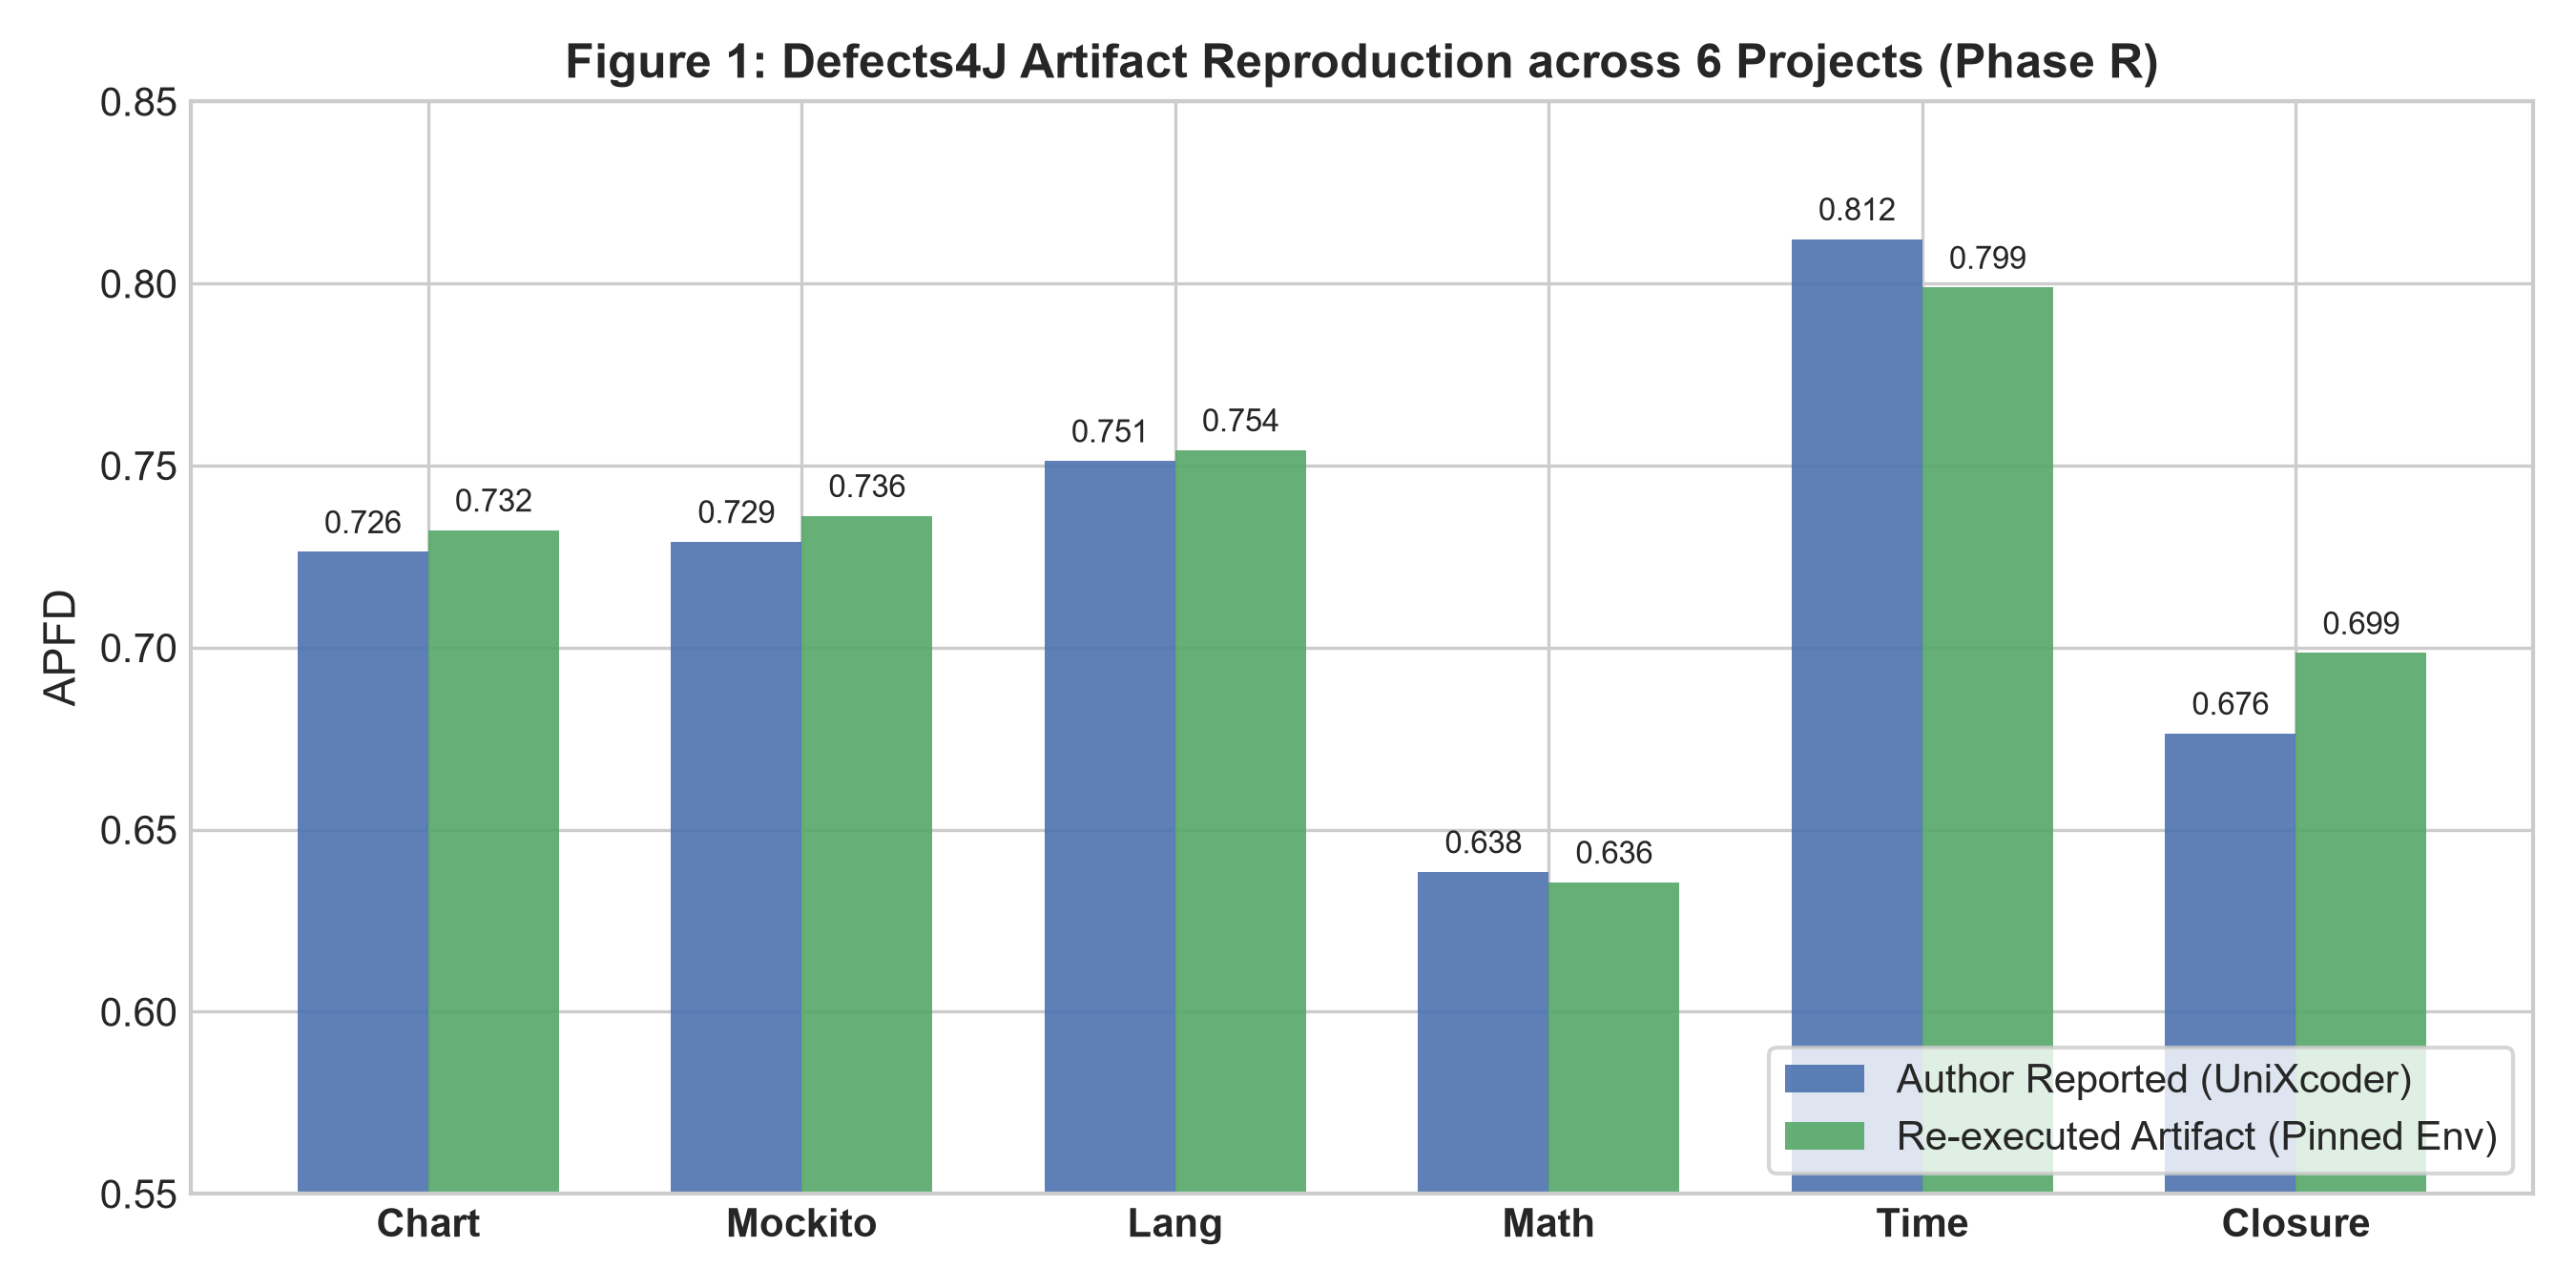
\includegraphics[width=0.85\textwidth]{Images/Figs/fig1_defects4j_reproduction.png}
\caption{So sánh điểm APFD giữa bài báo gốc FALCON và kết quả tái lập trên 6 dự án Defects4J}
\label{fig:defects4j_reproduction}
\vspace{1mm}
\footnotesize{\textit{Nguồn hình vẽ: Tệp kết xuất đồ họa \texttt{reports/figures/fig1\_defects4j\_reproduction.png}.}}
\end{figure}

% -----------------------------------------------------------------------------
\subsubsection{Phân tích phân rã kỹ thuật Bridge trên dự án Chart}
\label{subsubsec:bridge_chart}

Để xác định chính xác các yếu tố kỹ thuật tạo ra sự chênh lệch nhỏ trong tái lập, một thử nghiệm phân tách cấu trúc (Bridge experiment) gồm 4 nhánh (Arms) đã được thiết kế trên dự án Chart (26 phiên bản lỗi):
\begin{itemize}
    \item \textbf{Arm A (Base Pipeline):} Cài đặt cơ sở bám sát mô tả trong bài báo, không sử dụng clipping độ tương đồng.
    \item \textbf{Arm B (Cosine Clipping):} Cắt tỉa giá trị tương đồng cosin về khoảng $[0, 1]$ để ngăn ngừa giá trị âm.
    \item \textbf{Arm C (Greedy Sorting Variant):} Thay đổi quy tắc phá vỡ thế hòa (tie-breaking) trong thuật toán Greedy.
    \item \textbf{Arm D (Full Preprocessing Pipeline + Attention Mask):} Áp dụng tiền xử lý mã nguồn đầy đủ và sử dụng mặt nạ chú ý (attention mask) chuẩn của UniXcoder.
\end{itemize}

% nguon: reports/stage10/bridge/summary.json
Bảng~\ref{tab:bridge_chart_results} trình bày kết quả APFD thu được trên từng nhánh của thử nghiệm Bridge.

\begin{table}[H]
\centering
\caption{Kết quả phân rã các yếu tố kỹ thuật trong thử nghiệm Bridge trên dự án Chart}
\label{tab:bridge_chart_results}
\small
\begin{tabular}{llr}
\toprule
\textbf{Nhánh thử nghiệm} & \textbf{Cấu hình kỹ thuật} & \textbf{APFD trung bình} \\
\midrule
% nguon: reports/stage10/bridge/summary.json
Arm A & Base pipeline (không clipping) & 0,7323 \\
Arm B & Bổ sung Cosine Clipping $[0, 1]$ & 0,7323 \\
Arm C & Thay đổi quy tắc tie-breaking Greedy & 0,7323 \\
Arm D & Tiền xử lý mã nguồn + Attention Mask chuẩn & \textbf{0,7635} \\
\bottomrule
\end{tabular}
\vspace{1mm}\\
\footnotesize{\textit{Nguồn dữ liệu: Trích xuất từ tệp \texttt{reports/stage10/bridge/summary.json}. Chênh lệch giữa Arm D và Arm A đạt $+0,0312$ (+3,12 điểm phần trăm).}}
\end{table}

% nguon: reports/stage10/bridge/summary.json
Số liệu từ Bảng~\ref{tab:bridge_chart_results} ghi nhận điểm APFD trung bình giữ nguyên mức 0,7323 khi áp dụng clipping ma trận tương đồng (Arm B) hoặc thay đổi thứ tự phá vỡ thế hòa (Arm C). Tại nhánh Arm D (kết hợp tiền xử lý mã nguồn và mặt nạ chú ý chuẩn), điểm APFD trung bình đạt \textbf{0,7635}, tương ứng mức chênh lệch $+0,0312$ (+3,12 điểm phần trăm) so với Arm A.

Hình~\ref{fig:chart_bridge} thể hiện diễn biến điểm số qua 4 cấu hình của thử nghiệm Bridge.

\begin{figure}[H]
\centering
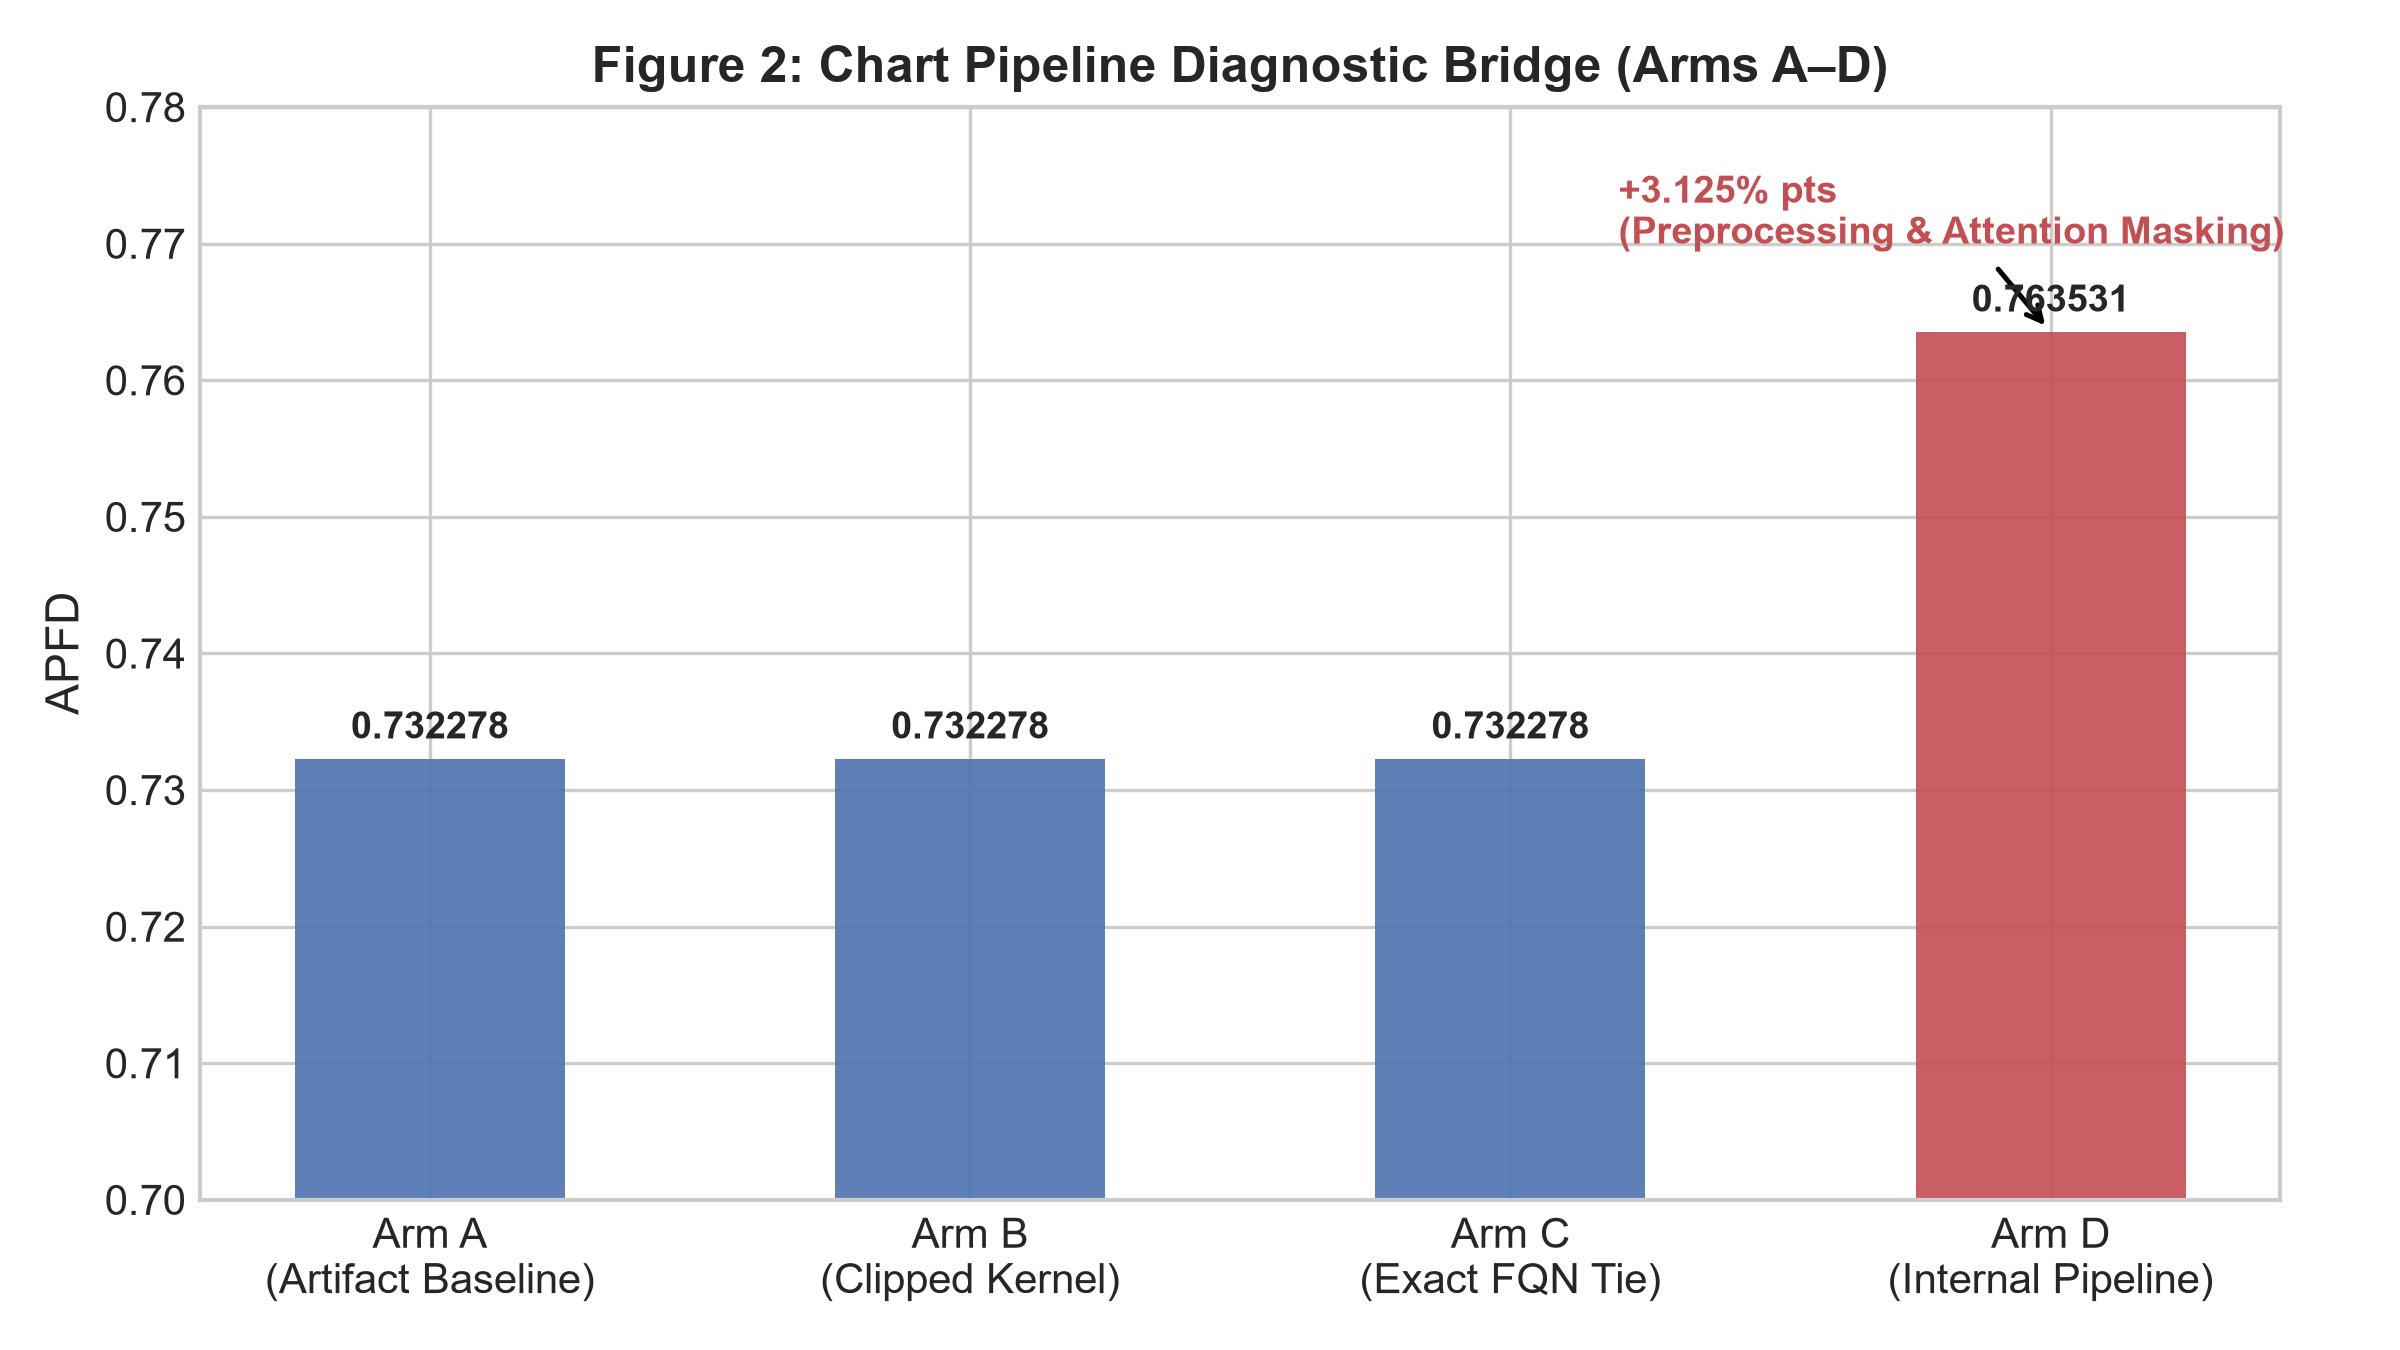
\includegraphics[width=0.85\textwidth]{Images/Figs/fig2_chart_bridge.png}
\caption{Phân rã ảnh hưởng của các thành phần kỹ thuật (Arm A--D) trên dự án Chart}
\label{fig:chart_bridge}
\vspace{1mm}
\footnotesize{\textit{Nguồn hình vẽ: Tệp kết xuất đồ họa \texttt{reports/figures/fig2\_chart\_bridge.png}.}}
\end{figure}

% -----------------------------------------------------------------------------
\subsubsection{Phát hiện kỹ thuật về Attention Mask}
\label{subsubsec:attention_mask_finding}

% nguon: reports/stage10/bridge/summary.json
Đối chiếu cấu hình giữa các nhánh thử nghiệm xác nhận sự thay đổi điểm số chỉ xuất hiện tại Arm D khi tích hợp tiền xử lý mã nguồn và truyền mặt nạ chú ý (attention mask) vào mô hình UniXcoder. Toàn bộ các thảo luận và phân tích cơ chế tác động của biểu diễn vector được trình bày tại Chương~\ref{sec:discussion}.

% =============================================================================
\subsection{Kết quả Trục 2: HC-FALCON trên hệ thống CI thực tế (LRTS)}
\label{subsec:rq2_lrts_results}

% -----------------------------------------------------------------------------
\subsubsection{Mốc đối chứng cơ sở ngẫu nhiên trên chuỗi thời gian CI}
\label{subsubsec:random_baseline_lrts}

% nguon: reports/stage6/karaf/summary.json, reports/stage6/activemq/summary.json, reports/stage6/log4j/summary.json, reports/stage12/ugcs_v2_absolute_apfdc.json
Trên tập Sàng lọc Phát triển (161 build lỗi), đường cơ sở ngẫu nhiên (\texttt{random}, trung bình qua 20 hạt giống ngẫu nhiên) ghi nhận điểm APFDc trung bình lần lượt là \textbf{0,4936} (trung vị 0,4908) tại Apache Karaf ($N=79$), \textbf{0,4945} (trung vị 0,4876) tại Apache ActiveMQ ($N=57$) và \textbf{0,4835} (trung vị 0,4897) tại Apache Log4j2 ($N=25$). Đường cơ sở thuần ngữ nghĩa (\texttt{fl\_only}) đạt điểm APFDc trung bình lần lượt là 0,4558 (Karaf), 0,5182 (ActiveMQ) và 0,6062 (Log4j2).

Bảng~\ref{tab:lrts_baseline_comparison} đối chiếu điểm APFDc trung bình giữa các đường cơ sở và các biến thể chính của đề tài trên chuỗi thời gian CI.

\begin{table}[H]
\centering
\caption{Đối chiếu điểm APFDc trung bình giữa các đường cơ sở và các biến thể chính trên CI}
\label{tab:lrts_baseline_comparison}
\small
\begin{adjustbox}{max width=\textwidth}
\begin{tabular}{lrrrr}
\toprule
\textbf{Phương pháp / Đường cơ sở} & \textbf{Karaf ($N=79$)} & \textbf{ActiveMQ ($N=57$)} & \textbf{Log4j2 ($N=25$)} & \textbf{Toàn bộ ($N=161$)} \\
\midrule
% nguon: reports/stage6/karaf/summary.json, reports/stage6/activemq/summary.json, reports/stage6/log4j/summary.json
Cơ sở ngẫu nhiên (\texttt{random})    & 0,4936 & 0,4945 & 0,4835 & 0,4923 \\
Thuần ngữ nghĩa (\texttt{fl\_only})   & 0,4558 & 0,5182 & 0,6062 & 0,5013 \\
Đường cơ sở \texttt{history\_cost}    & 0,7754 & 0,8486 & 0,8936 & 0,8197 \\
\midrule
% nguon: reports/release/statistical_tests_all_gens.json
HC-FALCON v1 (\texttt{normalized})   & 0,7710 & 0,8147 & 0,9014 & 0,8067 \\
% nguon: reports/stage12/ugcs_v2_absolute_apfdc.json
UGCS v2 (\texttt{hc\_ugcs\_v2})$^{*}$ & \textbf{0,7802} & \textbf{0,8471} & \textbf{0,8952} & \textbf{0,8217} \\
\bottomrule
\end{tabular}
\end{adjustbox}
\vspace{1mm}\\
\footnotesize{\textit{Nguồn dữ liệu: Tệp tổng hợp \texttt{reports/stage6/*/summary.json}, \texttt{reports/release/statistical\_tests\_all\_gens.json} và \texttt{reports/stage12/ugcs\_v2\_absolute\_apfdc.json}. ($*$) Điểm APFDc tuyệt đối của UGCS v2 được suy ra trực tiếp từ chênh lệch ghép cặp theo từng build vật lý: $\text{APFDc}(\text{UGCS v2})_i = \text{APFDc}(\text{history\_cost})_i + \Delta_i$.}}
\end{table}

Để so sánh đối chứng, biến thể khởi đầu HC-FALCON v1 (\texttt{normalized}) đạt điểm APFDc trung bình là \textbf{0,7710} tại Karaf, \textbf{0,8147} tại ActiveMQ và \textbf{0,9014} tại Log4j2; đường cơ sở \texttt{history\_cost} đạt điểm APFDc trung bình là \textbf{0,7754} tại Karaf, \textbf{0,8486} tại ActiveMQ và \textbf{0,8936} tại Log4j2. Biến thể cuối UGCS v2 đạt điểm APFDc trung bình suy ra lần lượt là \textbf{0,7802} tại Karaf, \textbf{0,8471} tại ActiveMQ và \textbf{0,8952} tại Log4j2 (trung bình toàn cục đạt \textbf{0,8217}). Mặc dù điểm APFDc trung bình của UGCS v2 tương đương \texttt{history\_cost}, việc phân tích kiểm định ghép cặp chi tiết theo từng bản build tại Mục~\ref{subsubsec:stage12_results} chỉ ra rằng UGCS v2 vẫn thua \texttt{history\_cost} ở 72,05\% số build vật lý.

% -----------------------------------------------------------------------------
\subsubsection{Diễn tiến các biến thể từ HC-FALCON v1 đến CNS-Greedy}
\label{subsubsec:variants_evolution}

Quá trình nghiên cứu trên tập Sàng lọc Phát triển (161 build lỗi) đã trải qua 4 thế hệ thuật toán liên tiếp:
\begin{enumerate}
    \item \textbf{Thế hệ 1 -- HC-FALCON v1 (Stage 6):} Bao gồm hai biến thể kết hợp tuyến tính giữa hàm Facility Location và trọng số lịch sử: dạng trọng số thô (\texttt{topic\_raw}) và dạng chuẩn hóa (\texttt{normalized}).
    % nguon: reports/release/statistical_tests.json (dòng 10, 25, 40)
    Biến thể chuẩn hóa ghi nhận trung vị $\Delta\text{APFDc}$ so với \texttt{history\_cost} lần lượt là $-1,2650$ điểm phần trăm (Karaf), $-1,4067$ điểm phần trăm (ActiveMQ) và $-0,1171$ điểm phần trăm (Log4j2).
    % nguon: reports/stage11/forensic-analysis.json (dòng 651-654)
    Trên toàn bộ 161 build lỗi, HC-FALCON v1 chỉ thắng 38 build (23,6\%), hòa 1 build (0,6\%) và thua 122 build (75,8\%).
    \item \textbf{Thế hệ 2 -- Hạn chế ngữ nghĩa theo cửa sổ lịch sử (Stage 8):} Giới hạn không gian tìm kiếm tham lam trong cửa sổ động theo từng bước với $q_b(i) \ge 0{,}95 \cdot q_b(t^*)$ và $c_b(i) \le 1{,}25 \cdot c_b(t^*)$ (neo theo phần tử đầu baseline $t^*$).
    % nguon: reports/stage8/summary.json
    Biến thể này ghi nhận: tại Karaf đạt 13 thắng / 17 hòa / 49 thua (trung vị $\Delta = -0,0171$ điểm phần trăm); tại ActiveMQ đạt 13 thắng / 1 hòa / 43 thua (trung vị $\Delta = -0,1537$ điểm phần trăm); tại Log4j2 đạt 5 thắng / 6 hòa / 14 thua (trung vị $\Delta = -0,0008$ điểm phần trăm). Tổng cộng trên 161 build lỗi, biến thể đạt 31 thắng / 24 hòa / 106 thua (thua 65,84\%).
    \item \textbf{Thế hệ 3 -- CNS-Greedy (Stage 11):} Can thiệp trực tiếp vào lợi ích biên kết hợp qua công thức $\text{gain}_{\text{CNS}}(i \mid S) = \alpha \cdot \frac{\Delta FL_b(i \mid S)}{n \cdot \sqrt{\max\left(c_b(i), \, 10^{-6}\right)}} + (1 - \alpha) \cdot w_b(i)$ với thời lượng thô $c_b(i)$ tính bằng giây và trọng số lịch sử chuẩn hóa $w_b(i) = q_b(i) / \sum q$.
    % nguon: reports/release/statistical_tests_all_gens.json (mục hc_cns_v1)
    Trên 161 build lỗi, CNS-Greedy đạt 22 thắng / 1 hòa / 56 thua tại Karaf (trung vị $\Delta = -0,3994$ điểm phần trăm), 10 thắng / 0 hòa / 47 thua tại ActiveMQ (trung vị $\Delta = -0,6064$ điểm phần trăm) và 6 thắng / 0 hòa / 19 thua tại Log4j2 (trung vị $\Delta = -0,1896$ điểm phần trăm). Tổng cộng đạt 38 thắng / 1 hòa / 122 thua (thua 75,78\%).
    \item \textbf{Thế hệ 4 -- UGCS v2 (Stage 12):} Biến thể tiền đăng ký kết hợp 4 công đoạn: Ước lượng Bayes $\to$ Khoanh vùng bất định $\to$ Tham lam có ý thức chi phí $\to$ Tie-breaking.
    % nguon: reports/stage12/stage12_statistical_tests_paired_effect_sizes.json
    Kết quả kiểm định ghi nhận: 20 thắng / 4 hòa / 55 thua tại Karaf (trung vị $\Delta = -0,0586$ điểm phần trăm), 9 thắng / 4 hòa / 44 thua tại ActiveMQ (trung vị $\Delta = -0,2235$ điểm phần trăm) và 6 thắng / 2 hòa / 17 thua tại Log4j2 (trung vị $\Delta = -0,0017$ điểm phần trăm). Tổng cộng đạt 35 thắng / 10 hòa / 116 thua (thua 72,05\%).
\end{enumerate}

% nguon: reports/stage12/winning_builds_intersection.json
Đối soát giao thoa các tập build thắng giữa các thế hệ thuật toán xác nhận:
\begin{itemize}
    \item \textbf{Giữa Stage 6 (v1) và Stage 8 (Hạn chế ngữ nghĩa):} Stage 8 giữ lại 15 trong số 38 ca thắng của v1 (39,5\%), đồng thời mở ra thêm 16 ca thắng mới mà v1 không đạt được. Số liệu này bác bỏ giả thuyết cho rằng Stage 8 bóp nghẹt toàn bộ các ca thắng của v1.
    \item \textbf{Giữa Stage 6 (v1) và Stage 11 (CNS-Greedy):} Mặc dù cả hai biến thể cùng đạt chính xác 38 build thắng trên toàn bộ 161 build lỗi, hai tập hợp build thắng này không trùng khớp nhau ($\text{Wins}_{v1} \neq \text{Wins}_{\text{cns}}$). Chúng chỉ giao thoa 23 build chung (60,5\%), mỗi biến thể sở hữu 15 ca thắng độc lập còn lại.
    \item \textbf{Tính bền vững qua 4 thế hệ:} Có đúng 14 build lỗi duy trì được chiến thắng trước \texttt{history\_cost} xuyên suốt từ biến thể khởi đầu v1 tới biến thể cuối UGCS v2.
\end{itemize}

% -----------------------------------------------------------------------------
\subsubsection{Kết quả của biến thể cuối UGCS v2 (Stage 12)}
\label{subsubsec:stage12_results}

Bảng~\ref{tab:stage12_comprehensive} trình bày chi tiết kết quả kiểm định thống kê và các chỉ số kích thước hiệu ứng của biến thể cuối UGCS v2 so với đường cơ sở \texttt{history\_cost} trên tập Sàng lọc Phát triển.

\begin{table}[H]
\centering
\caption{Kết quả kiểm định thống kê ghép cặp giữa UGCS v2 và baseline \texttt{history\_cost}}
\label{tab:stage12_comprehensive}
\begin{adjustbox}{max width=\textwidth}
\small
\begin{tabular}{lrrr}
\toprule
\textbf{Chỉ số thống kê} & \textbf{Apache Karaf} & \textbf{Apache ActiveMQ} & \textbf{Apache Log4j2} \\
\midrule
% nguon: reports/stage12/stage12_statistical_tests_paired_effect_sizes.json
Số lượng physical build lỗi ($N$) & 79 & 57 & 25 \\
Số build Thắng / Thua / Hòa & 20 / 55 / 4 & 9 / 44 / 4 & 6 / 17 / 2 \\
Tỷ lệ thắng (Win rate) & 25,32\% & 15,79\% & 24,00\% \\
\midrule
% nguon: reports/stage12/stage12_statistical_tests.json
Trung vị chênh lệch ($\text{Median}(\Delta)$, điểm phần trăm) & \textbf{$-0,0586$} & \textbf{$-0,2235$} & \textbf{$-0,0017$} \\
Trung bình chênh lệch ($\text{Mean}(\Delta)$, điểm phần trăm)   & \textbf{$+0,4788$} & \textbf{$-0,1508$} & \textbf{$+0,1663$} \\
Khoảng tin cậy Bootstrap 95\% (điểm phần trăm) & [$-0,2659, +1,4488$] & [$-0,8112, +0,6703$] & [$-0,1606, +0,6060$] \\
\midrule
% nguon: reports/stage12/stage12_statistical_tests.json
Wilcoxon $W$-statistic & 1.067,0 & 318,0 & 113,0 \\
Giá trị $p$ chưa hiệu chỉnh ($p_{\text{raw}}$) & 0,012684 & $6,30 \times 10^{-5}$ & 0,187317 \\
Giá trị $p$ hiệu chỉnh Holm ($p_{\text{holm}}$) & \textbf{0,025368} & \textbf{0,000189} & \textbf{0,187317} \\
\midrule
% nguon: reports/stage12/stage12_statistical_tests_paired_effect_sizes.json
Paired Cliff's delta ($\delta_{\text{paired}}$) & \textbf{$-0,4430$} & \textbf{$-0,6140$} & \textbf{$-0,4400$} \\
Rank-biserial correlation ($r_{rb}$) & \textbf{$-0,3102$} & \textbf{$-0,6059$} & \textbf{$-0,2681$} \\
\bottomrule
\end{tabular}
\end{adjustbox}
\vspace{1mm}\\
\footnotesize{\textit{Nguồn dữ liệu: Tệp kiểm định \texttt{reports/stage12/stage12\_statistical\_tests\_paired\_effect\_sizes.json}. Chú ý thống kê: Trung vị của hiệu khác hiệu của các trung vị ($\text{Median}(X - Y) \neq \text{Median}(X) - \text{Median}(Y)$). Do đó, việc trung vị chênh lệch ghép cặp $\text{Median}(\Delta)$ mang dấu âm (do đa số các build có hiệu âm) hoàn toàn tương thích về mặt toán học với việc hiệu của hai trung vị mẫu hoặc giá trị trung bình $\text{Mean}(\Delta)$ mang dấu dương (bị chi phối bởi một số ít build có mức chênh lệch dương lớn).}}
\end{table}

Số liệu từ Bảng~\ref{tab:stage12_comprehensive} chỉ ra các hiện tượng thống kê cụ thể:
\begin{enumerate}
    \item \textbf{Hiện tượng phân kỳ dấu giữa Median và Mean tại Apache Karaf:}
    % nguon: reports/stage12/stage12_statistical_tests.json
    Tại Karaf, giá trị trung vị chênh lệch mang dấu âm ($-0,0586$ điểm phần trăm, với 20 build thắng, 55 build thua và 4 build hòa), trong khi giá trị trung bình chênh lệch mang dấu dương ($+0,4788$ điểm phần trăm). Cần nhấn mạnh nguyên lý thống kê: trung vị của hiệu khác hiệu của các trung vị ($\text{Median}(\Delta) \neq \text{Median}_{\text{cand}} - \text{Median}_{\text{base}}$). Khoảng tin cậy Bootstrap 95\% của giá trị trung bình trải rộng từ $-0,2659$ đến $+1,4488$ điểm phần trăm (chứa mốc 0), cho thấy sự khác biệt trung bình không đạt ý nghĩa thống kê ở mức $\alpha = 0,05$.
    \item \textbf{Mức độ thua thiệt tại Apache ActiveMQ:}
    Tại ActiveMQ, cả trung vị ($-0,2235$ điểm phần trăm) và trung bình ($-0,1508$ điểm phần trăm) đều mang dấu âm, với tỷ lệ thắng chỉ đạt 15,79\% (9 thắng vs 44 thua). Kiểm định Wilcoxon đạt mức ý nghĩa thống kê rất cao ($p_{\text{holm}} = 0,000189 < 0,001$). Các chỉ số kích thước hiệu ứng ghép cặp ghi nhận mức bất lợi lớn: Paired Cliff's delta đạt $-0,6140$ và Rank-biserial đạt $-0,6059$.
    \item \textbf{Thiếu ý nghĩa thống kê tại Apache Log4j2:}
    Tại Log4j2 ($N=25$), tỷ số thắng/thua là 6/17, trung vị đạt $-0,0017$ điểm phần trăm, giá trị $p$ hiệu chỉnh Holm đạt 0,187317 ($> 0,05$) và khoảng tin cậy 95\% chứa mốc 0 ([$-0,1606, +0,6060$] điểm phần trăm).
\end{enumerate}

Hình~\ref{fig:lrts_effect_gate} minh họa phân phối chênh lệch ghép cặp $\Delta\text{APFDc}$ của UGCS v2 so với hai đường cơ sở đối chứng trên cả 3 dự án.

\begin{figure}[H]
\centering
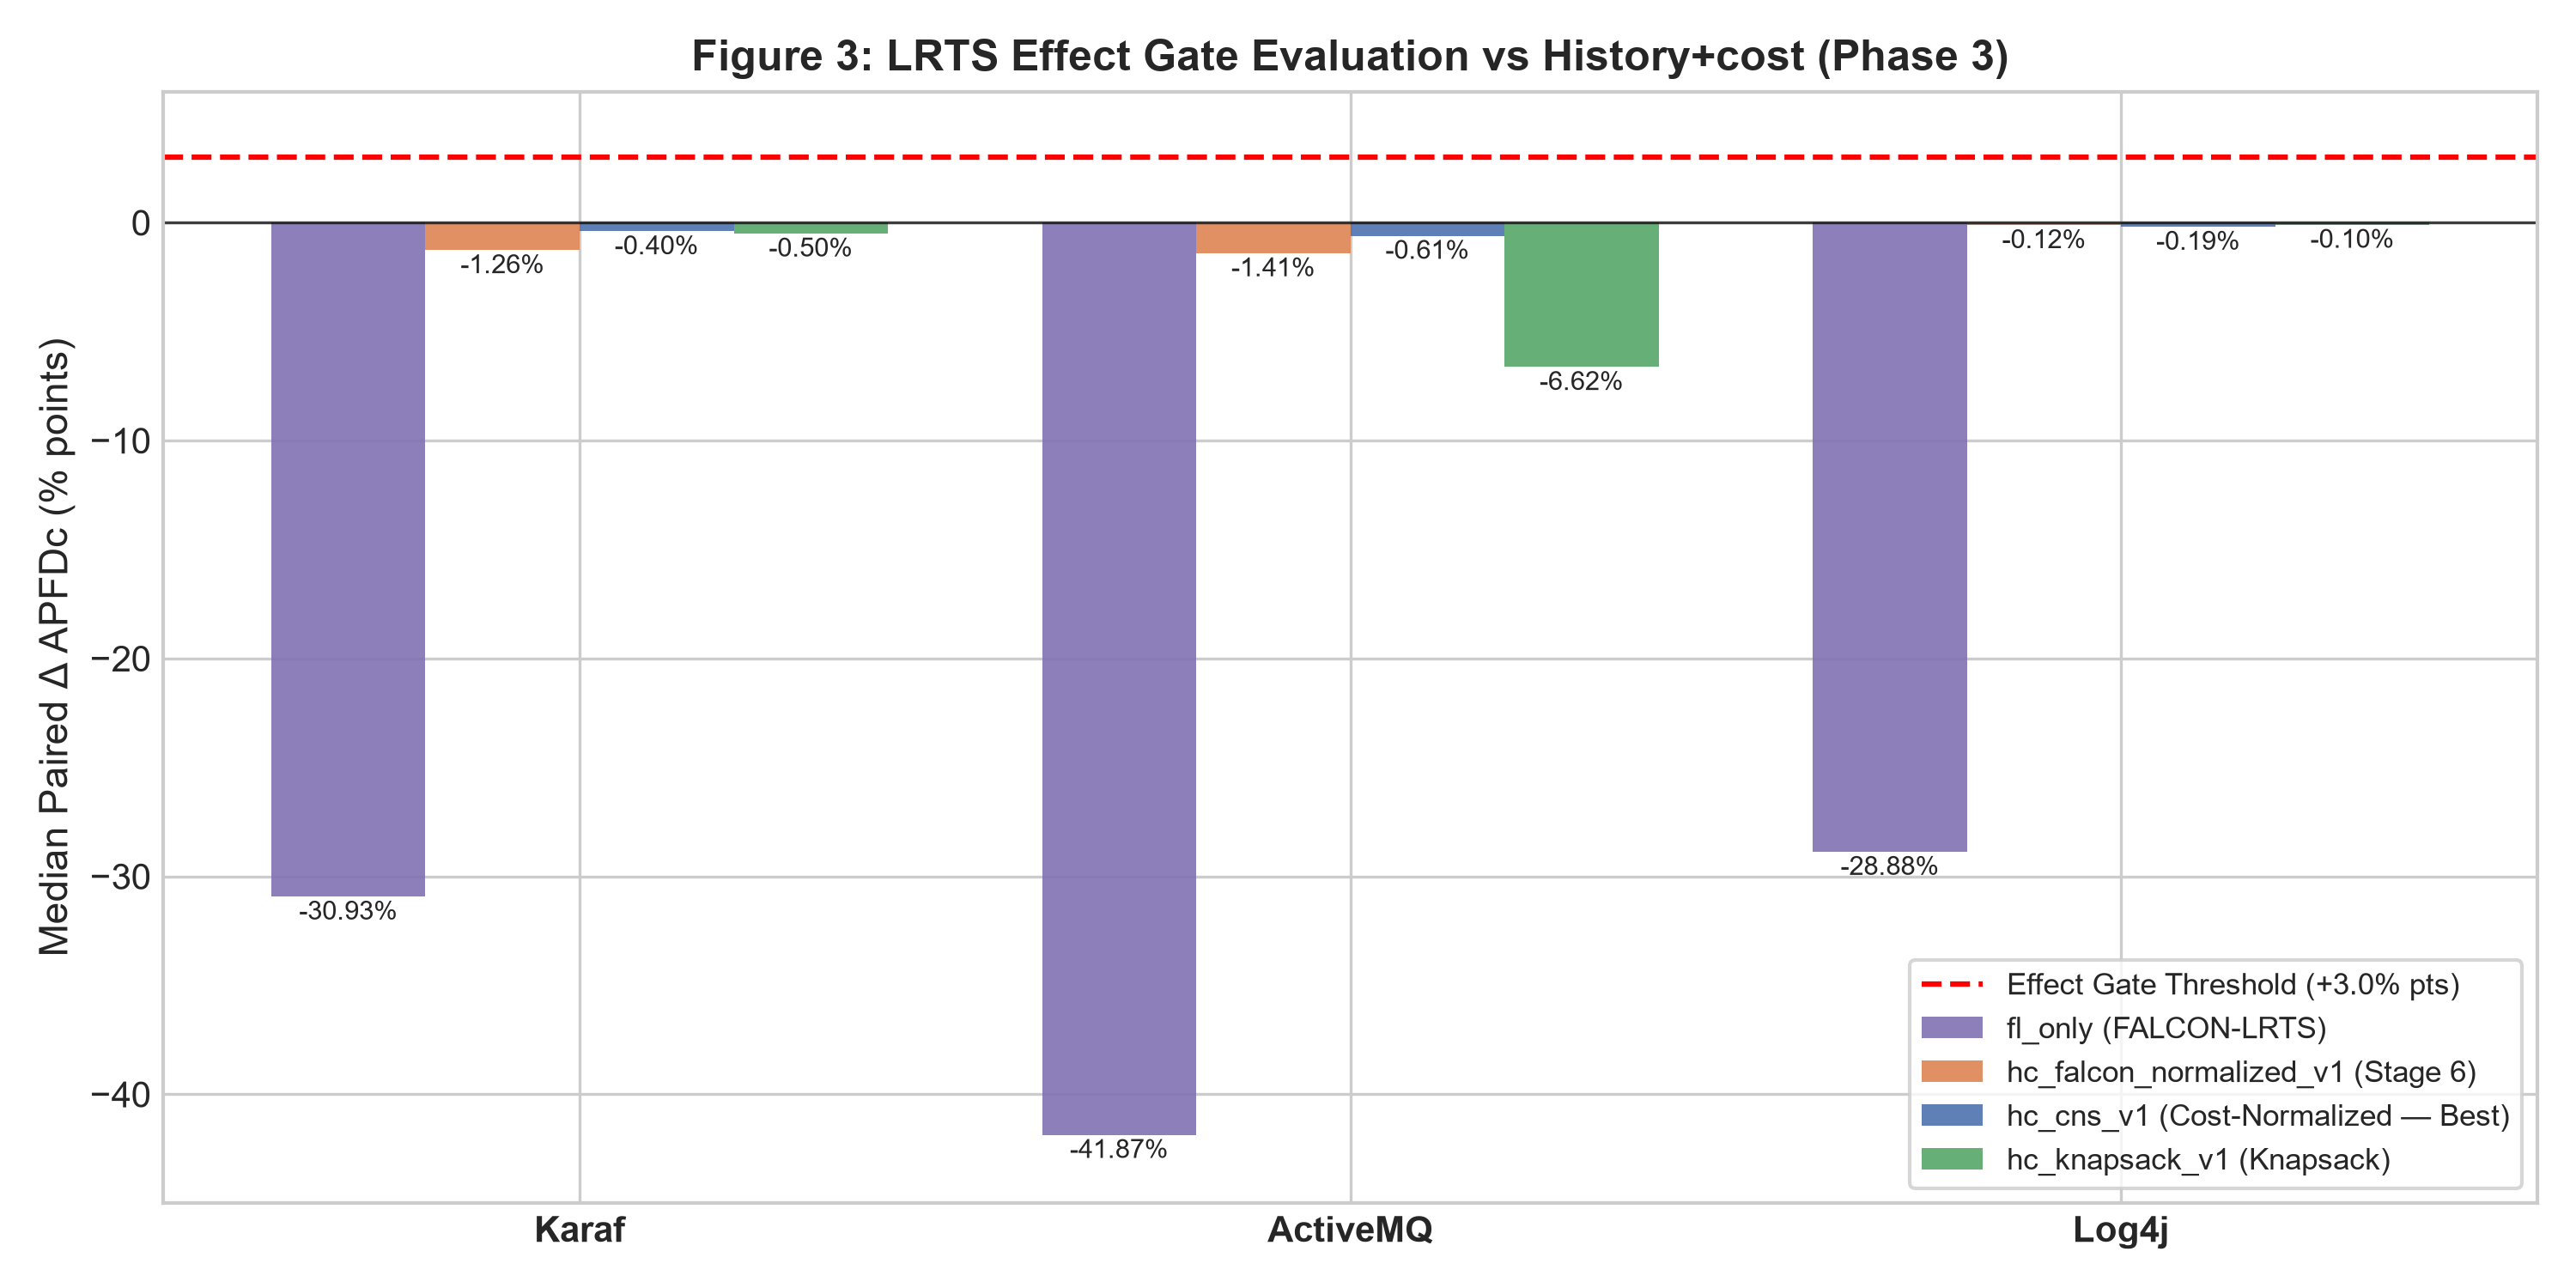
\includegraphics[width=0.85\textwidth]{Images/Figs/fig3_lrts_effect_gate.png}
\caption[Phân phối chênh lệch ghép cặp $\Delta\text{APFDc}$ của UGCS v2 so với các baseline]{Phân phối chênh lệch ghép cặp $\Delta\text{APFDc}$ của UGCS v2 so với \texttt{history\_cost} và \texttt{fl\_only}}
\label{fig:lrts_effect_gate}
\vspace{1mm}
\footnotesize{\textit{Nguồn hình vẽ: Tệp kết xuất đồ họa \texttt{reports/figures/fig3\_lrts\_effect\_gate.png}. Đường nét đứt màu đỏ biểu thị ngưỡng yêu cầu $+3,0$ điểm phần trăm của Effect Gate.}}
\end{figure}

% -----------------------------------------------------------------------------
\subsubsection{Đánh giá các chỉ tiêu kỹ thuật (Overhead thời gian và Bộ nhớ)}
\label{subsubsec:engineering_metrics}

% nguon: reports/stage12/development-screen.json (dòng 85-113)
Bên cạnh hiệu quả phát hiện lỗi, đề tài đã tiến hành đo đạc chính xác các chỉ tiêu kỹ thuật thực thi của UGCS v2 so với đường cơ sở \texttt{history\_cost} trên toàn bộ 171 stage thuộc 161 build lỗi của tập Sàng lọc Phát triển:
\begin{itemize}
    % nguon: reports/stage12/development-screen.json (dòng 111, 112)
    \item \textbf{Độ trễ tính toán mỗi stage (Latency per stage):} Baseline nhẹ \texttt{history\_cost} có thời gian xếp hạng cực nhanh với độ trễ trung vị chỉ \textbf{0,11 ms} ($0,0001126$ giây). Ngược lại, việc giải bài toán chọn tập con tham lam có nhận thức chi phí kết hợp nhân cosin ngữ nghĩa của UGCS v2 đòi hỏi độ trễ trung vị là \textbf{53,82 ms} ($0,053819$ giây), tức chậm hơn xấp xỉ 478 lần ở mức trung vị.
    % nguon: reports/stage12/development-screen.json (dòng 89, 109)
    \item \textbf{Tỷ lệ overhead trần ở phân vị P95 (P95 warm overhead fraction):} Tỷ lệ gia tăng chi phí thời gian xếp hạng ở phân vị thứ 95 của UGCS v2 so với \texttt{history\_cost} lên tới \textbf{14.257,90 lần} ($+1.425.790\%$). Mức overhead tính toán vượt xa ngưỡng trần cho phép $+10\%$ ($0,10$), dẫn tới việc phương pháp vi phạm hoàn toàn Runtime Gate.
    % nguon: reports/stage12/development-screen.json (dòng 95, 110)
    \item \textbf{Mức chiếm dụng bộ nhớ đỉnh (Peak RSS):} Mức tiêu thụ bộ nhớ RAM cao nhất của tiến trình xếp hạng ghi nhận tại \textbf{656,4 MiB} ($688.287.744$ bytes), nằm an toàn dưới ngưỡng trần tiền đăng ký là 8,0 GiB ($8.589.934.592$ bytes).
    \item \textit{Ghi chú đối soát dữ liệu:} Các phân vị cụ thể khác (P95 tuyệt đối, Max) của thời gian chạy từng build vật lý cũng như của biến thể HC-FALCON v1 không xác định được từ tệp \texttt{reports/stage12/development-screen.json} do tệp nguồn chỉ lưu trữ trung vị độ trễ của hai phương pháp và tỷ lệ trần P95 toàn cục.
\end{itemize}

% -----------------------------------------------------------------------------
\subsubsection{Phán quyết thẩm định theo tiêu chí tiền đăng ký}
\label{subsubsec:preregistered_decision}

% nguon: reports/stage12/development-screen.json (dòng 10-104), configs/hc-falcon-v2-preregistered.json (dòng 42-69)
Bảng~\ref{tab:decision_gates_evaluation} tổng hợp kết quả đối chiếu toàn bộ 4 cổng quyết định tiền đăng ký đối với biến thể cuối UGCS v2 trên tập Sàng lọc Phát triển.

\begin{table}[H]
\centering
\caption{Đánh giá các cổng quyết định tiền đăng ký (Decision Gates) đối với biến thể UGCS v2}
\label{tab:decision_gates_evaluation}
\small
\begin{adjustbox}{max width=\textwidth}
\begin{tabular}{llp{5.5cm}ll}
\toprule
\textbf{Cổng thẩm định} & \textbf{Chỉ số đánh giá} & \textbf{Ngưỡng tiền đăng ký} & \textbf{Giá trị quan sát} & \textbf{Kết luận} \\
\midrule
% nguon: reports/stage12/development-screen.json (dòng 15-20)
Effect Gate      & $\Delta\text{APFDc}$ vs baseline & $\ge +3,0$ điểm phần trăm trên $\ge 2/3$ dự án so với \texttt{history\_cost} và \texttt{fl\_only} & 0/3 dự án đạt chuẩn so với \texttt{history\_cost} & \textbf{KHÔNG ĐẠT} \\
% nguon: reports/stage12/development-screen.json (dòng 86-90)
Runtime Gate     & Overhead thời gian P95          & Tỷ lệ gia tăng chi phí $\le 0,10$ ($+10\%$) vs \texttt{history\_cost} & $14.257,90\times$ ($+1.425.790\%$) & \textbf{VI PHẠM} \\
% nguon: reports/stage12/development-screen.json (dòng 92-96)
Memory Gate      & Mức chiếm dụng đỉnh (Peak RSS)   & Dung lượng RAM $\le 8{,}0$ GiB ($8.589.934.592$ bytes) & 656,4 MiB ($688.287.744$ bytes) & \textbf{ĐẠT} \\
% nguon: reports/stage12/development-screen.json (dòng 98-102)
Audit Gate       & Tính toàn vẹn và lỗi thực thi   & Hoàn thành 171 stage trên 161 build, không có lỗi & 171/171 stage, 0 lỗi audit & \textbf{ĐẠT} \\
\midrule
% nguon: reports/stage12/development-screen.json (dòng 10, 7)
\textbf{Phán quyết chung} & \textbf{Quyết định phát hành} & \textbf{Vượt qua toàn bộ 4 cổng} & \textbf{Vi phạm 2/4 cổng} & \textbf{NO-GO} \\
\bottomrule
\end{tabular}
\end{adjustbox}
\vspace{1mm}\\
\footnotesize{\textit{Nguồn dữ liệu: Tệp thẩm định chính thức \texttt{reports/stage12/development-screen.json}.}}
\end{table}

% nguon: docs/12-hc-falcon-v2/evaluation-protocol.md (dòng 104-117)
Đối chiếu với các điều kiện tiền đăng ký, phương pháp đạt 2 cổng kỹ thuật (Memory Gate và Audit Gate) nhưng thất bại tại 2 cổng cốt lõi (Effect Gate và Runtime Gate). Cụ thể, mẫu số chuẩn hóa của chỉ số overhead được quy định nghiêm ngặt là thời gian xếp hạng của đường cơ sở \texttt{history\_cost}:
\begin{equation}
\text{Overhead}_{\text{stage}} = \frac{T_{\text{ugcs}} - T_{\text{hc}}}{\max(T_{\text{hc}}, 10^{-9})}
\end{equation}
Do độ trễ trung vị của \texttt{history\_cost} chỉ là 0,11 ms trong khi UGCS v2 tiêu tốn 53,82 ms, tỷ lệ overhead P95 quan sát lên tới $14.257,90\times$ ($+1.425.790\%$), vượt xa ngưỡng cho phép $+10\%$. Đồng thời, tại Effect Gate, UGCS v2 không đạt mức tăng trưởng $+3,0$ điểm phần trăm so với \texttt{history\_cost} trên bất kỳ dự án nào (0/3 dự án).

Căn cứ theo quy tắc phán quyết đã khóa cứng trước thực nghiệm, kết luận chính thức của đề tài là \textbf{NO-GO}. Hệ thống kích hoạt lệnh đóng băng: \textbf{Toàn bộ 142 build lỗi thuộc tập Xác nhận Niêm phong (Reserved Confirmation) được giữ niêm phong vĩnh viễn (\texttt{reserved\_opened: false})}, bảo đảm tính toàn vẹn phương pháp luận và ngăn ngừa triệt để hiện tượng rò rỉ dữ liệu kiểm chứng.

% =============================================================================
\subsection{Dữ liệu chẩn đoán sâu về hiện tượng Heavy Predecessors}
\label{subsec:rq3_heavy_predecessors}

% -----------------------------------------------------------------------------
\subsubsection{Thống kê độ trễ ròng tích lũy trên 161 build lỗi}
\label{subsubsec:forensic_table}

Để cung cấp bằng chứng thực nghiệm trực tiếp giải thích sự sụt giảm APFDc của các mô hình kết hợp ngữ nghĩa, phân tích điều tra sâu (forensic analysis) đã đo đạc sự dịch chuyển vị trí thực thi của các test class trên toàn bộ 161 build lỗi của biến thể HC-FALCON v1 (\texttt{normalized\_v1}) so với \texttt{history\_cost}.

% nguon: reports/stage12/predecessor_comparison.json, reports/stage11/forensic-analysis.json
Bảng~\ref{tab:heavy_predecessors_breakdown} phân rã chi tiết tổng thời gian các bài test nặng bị đẩy lên trước test lỗi ($T_{add}$), thời gian test lỗi được đẩy lên trước ($T_{rem}$) và độ trễ ròng tích lũy ($T_{net} = T_{add} - T_{rem}$) giữa hai biến thể HC-FALCON v1 và UGCS v2 theo từng dự án. Cả hai biến thể đều được tính toán theo cùng một định nghĩa toán học nhất quán trên 161 build vật lý (171 failing stages) đối chiếu trực tiếp với baseline \texttt{history\_cost}.

\begin{table}[H]
\centering
\caption{Đối chiếu phân rã thời gian trễ do Heavy Predecessors giữa HC-FALCON v1 và UGCS v2}
\label{tab:heavy_predecessors_breakdown}
\small
\begin{adjustbox}{max width=\textwidth}
\begin{tabular}{llrrrrr}
\toprule
\textbf{Biến thể} & \textbf{Dự án CI} & \textbf{Build ($N$)} & \textbf{$T_{add}$ (s)} & \textbf{$T_{rem}$ (s)} & \textbf{$T_{net}$ (s)} & $\mathbf{T_{net}/N}$ \textbf{(s)} \\
\midrule
% nguon: reports/stage12/predecessor_comparison.json (mục hc_falcon_normalized_v1)
\multirow{4}{*}{\textbf{HC-FALCON v1}} 
  & Apache Karaf   & 79 & $+18.205,5$ & $-23.384,8$ & $\mathbf{-5.179,3}$ & $-65,56$ \\
  & Apache ActiveMQ & 57 & $+115.759,2$ & $-71.872,9$ & $\mathbf{+43.886,3}$ & $+769,94$ \\
  & Apache Log4j2  & 25 & $+1.027,2$ & $-635,0$ & $\mathbf{+392,2}$ & $+15,69$ \\
\cmidrule{2-7}
  & \textbf{Tổng cộng v1} & \textbf{161} & $\mathbf{+134.991,9}$ & $\mathbf{-95.892,7}$ & $\mathbf{+39.099,3}$ & $\mathbf{+242,85}$ \\
\midrule
% nguon: reports/stage12/predecessor_comparison.json (mục hc_ugcs_v2)
\multirow{4}{*}{\textbf{UGCS v2}} 
  & Apache Karaf   & 79 & $+4.858,5$ & $-11.378,1$ & $\mathbf{-6.519,6}$ & $-82,53$ \\
  & Apache ActiveMQ & 57 & $+38.644,6$ & $-41.746,1$ & $\mathbf{-3.101,4}$ & $-54,41$ \\
  & Apache Log4j2  & 25 & $+196,2$ & $-206,4$ & $\mathbf{-10,2}$ & $-0,41$ \\
\cmidrule{2-7}
  & \textbf{Tổng cộng UGCS v2} & \textbf{161} & $\mathbf{+43.699,3}$ & $\mathbf{-53.330,6}$ & $\mathbf{-9.631,3}$ & $\mathbf{-59,82}$ \\
\bottomrule
\end{tabular}
\end{adjustbox}
\vspace{1mm}\\
\footnotesize{\textit{Nguồn dữ liệu: Tệp tổng hợp đối soát \texttt{reports/stage12/predecessor\_comparison.json}. Cả hai biến thể được đo đạc bằng cùng một hàm toán học trên 161 build lỗi (171 failing stages). Đối với HC-FALCON v1, tổng độ trễ ròng tích lũy ghi nhận $+39.099,3$ giây; đối với UGCS v2, tổng thời gian ròng ghi nhận mức cắt giảm $-9.631,3$ giây so với \texttt{history\_cost}. Cột $T_{net}/N$ thể hiện độ trễ ròng bình quân trên mỗi bản build vật lý.}}
\end{table}

Số liệu đối chiếu từ Bảng~\ref{tab:heavy_predecessors_breakdown} chỉ ra các phát hiện cốt lõi:
\begin{itemize}
    \item \textbf{Ở biến thể khởi đầu HC-FALCON v1:} Hiện tượng Heavy Predecessors bộc lộ rất nghiêm trọng tại Apache ActiveMQ ($T_{net} = +43.886,3$ giây, trung bình $+769,94$ s/build) và Log4j2 ($T_{net} = +392,2$ giây, trung bình $+15,69$ s/build). Trên toàn bộ 161 build lỗi, tổng thời gian bị trễ thêm là $+39.099,3$ giây (bình quân $+242,85$ s/build).
    \item \textbf{Ở biến thể cải tiến UGCS v2:} Nhờ cơ chế khoanh vùng bất định và chuẩn hóa chi phí nghiêm ngặt, UGCS v2 đã khống chế hoàn toàn hiện tượng Heavy Predecessors ở quy mô tổng thể: giá trị độ trễ ròng $T_{net}$ mang dấu âm trên cả 3 dự án (Karaf: $-6.519,6$ s, tức $-82,53$ s/build; ActiveMQ: $-3.101,4$ s, tức $-54,41$ s/build; Log4j2: $-10,2$ s, tức $-0,41$ s/build), đạt mức cắt giảm ròng tổng cộng \textbf{$-9.631,3$ giây} (bình quân $-59,82$ s/build) thời gian chờ test lỗi đầu tiên so với \texttt{history\_cost}.
    \item \textbf{Mối tương quan giữa độ trễ ròng $T_{net}$ và tỷ lệ thua theo build:} Mặc dù UGCS v2 đã cắt giảm thành công độ trễ ròng từ $+39.099,3$ s xuống $-9.631,3$ s trên quy mô toàn tập, biến thể này vẫn ghi nhận điểm APFDc thấp hơn \texttt{history\_cost} ở đa số các bản build vật lý (thua 116/161 build, tương đương 72,05\% toàn tập; thua 55/79 tại Karaf, 44/57 tại ActiveMQ và 17/25 tại Log4j2).
\end{itemize}

Hình~\ref{fig:heavy_predecessors} minh họa tương quan phân rã giữa $T_{add}$, $T_{rem}$ và độ trễ ròng tích lũy $T_{net}$ trên 3 dự án.

\begin{figure}[H]
\centering
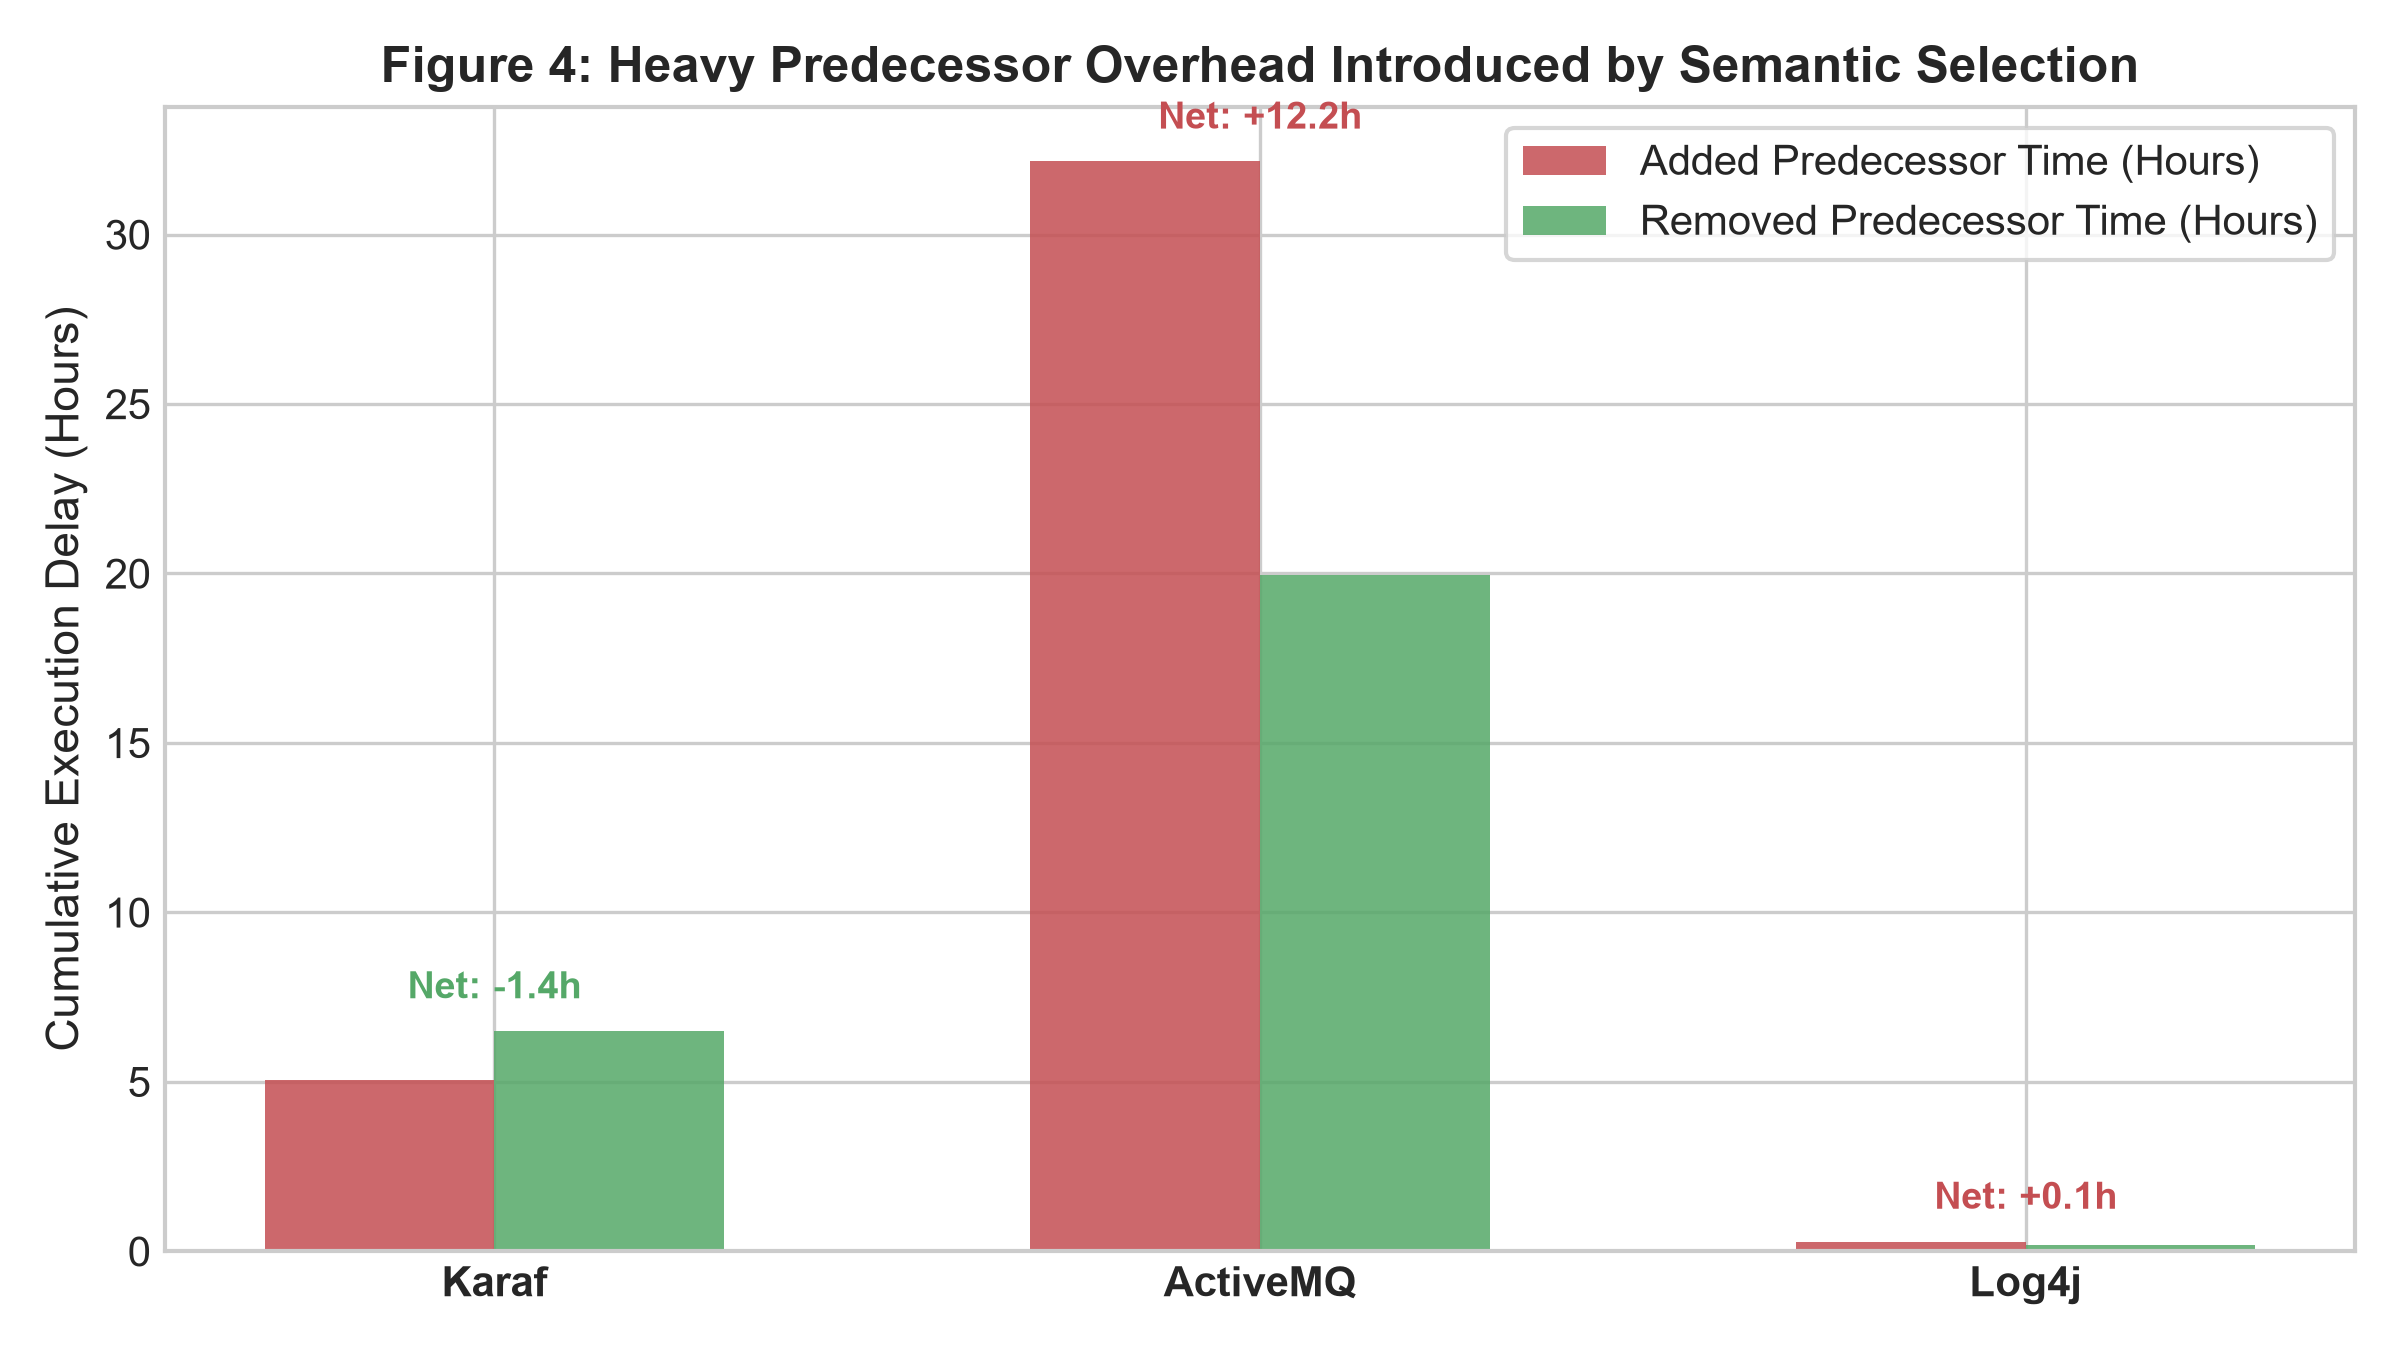
\includegraphics[width=0.85\textwidth]{Images/Figs/fig4_heavy_predecessors.png}
\caption{Phân rã độ trễ tích lũy ($T_{add}$, $T_{rem}$, $T_{net}$) do hiện tượng Heavy Predecessors}
\label{fig:heavy_predecessors}
\vspace{1mm}
\footnotesize{\textit{Nguồn hình vẽ: Tệp kết xuất đồ họa \texttt{reports/figures/fig4\_heavy\_predecessors.png}.}}
\end{figure}

% -----------------------------------------------------------------------------
\subsubsection{Các lớp kiểm thử đóng vai trò thủ phạm gây trễ điển hình}
\label{subsubsec:top_heavy_predecessors}

Phân tích chi tiết mức độ dịch chuyển cho thấy hiện tượng trễ tập trung vào một số lớp kiểm thử cụ thể có thời gian chạy dài:
\begin{itemize}
    % nguon: reports/stage11/forensic-analysis.json (dòng 319-320)
    \item Lớp kiểm thử \texttt{MQTTAutoNioTest} (ActiveMQ): Có thời gian thực thi trung bình từ 150 đến 250 giây. Trong thứ tự xếp hạng của HC-FALCON v1, bài test này xuất hiện làm Heavy Predecessor trong \textbf{102 lượt} (failure shifts) trải dài trên \textbf{38 trong tổng số 57 build lỗi} (66,7\%) của ActiveMQ.
    % nguon: reports/stage11/forensic-analysis.json (dòng 324)
    \item Lớp kiểm thử \texttt{StompAutoNioSslTest} (ActiveMQ): Xuất hiện làm Heavy Predecessor trong \textbf{76 lượt} trên hệ thống CI của ActiveMQ.
    % nguon: docs/BAO_CAO_TONG_HOP_DU_AN.md (dòng 462, 463)
    \item Tại Karaf: hai lớp kiểm thử \texttt{Spring43FeaturesTest} và \texttt{SystemCommandSecurityTest} lần lượt xuất hiện làm tiền nhiệm đứng trước các test phát hiện lỗi trong \textbf{42 lượt} và \textbf{40 lượt}.
    % nguon: docs/BAO_CAO_TONG_HOP_DU_AN.md (dòng 469)
    \item Lớp kiểm thử \texttt{RollingAppenderDirectWriteTest} (Log4j2): Xuất hiện làm tiền nhiệm gây trễ trong \textbf{24 lượt} tại Log4j2.
\end{itemize}

% =============================================================================
\subsection{Phân tích bóc tách các thành phần (Ablation Study)}
\label{subsec:ablation}

% TODO: Hiện tại trong kho dữ liệu chưa ghi nhận thực nghiệm bóc tách độc lập (ablation study) riêng rẽ cho từng hệ số phạt chi phí hay kịch bản cold-start độc lập. Mục này được tạm thời giữ nguyên cấu trúc nháp để bổ sung khi có dữ liệu.

Hiện tại, các thực nghiệm đối chứng bóc tách thành phần độc lập (như việc ngắt bỏ hoàn toàn hệ số chi phí hay cô lập tín hiệu ngữ nghĩa trong giai đoạn khởi động lạnh cold-start) chưa được hoàn thiện trên kho lưu trữ. Các phát hiện định lượng liên quan sẽ được bổ sung khi có dữ liệu thực nghiệm kiểm chứng độc lập.

% =============================================================================
\subsection{Tổng kết chương}
\label{subsec:experiments_summary}

Chương 4 đã báo cáo toàn diện các số liệu thực nghiệm thu được từ hai trục nghiên cứu:
\begin{enumerate}
    \item \textbf{Trên Defects4J (Trục 1):} Tái lập thuật toán FALCON trên 6 dự án phần mềm với điểm APFD trung bình đạt 0,7260 so với 0,7223 của bài báo gốc (sai lệch có dấu trung bình $+0,0037$, sai lệch tuyệt đối trung bình MAE đạt $0,0042$, sai lệch tuyệt đối lớn nhất là $0,0132$ tại Math). Thử nghiệm Bridge xác nhận việc bổ sung tiền xử lý mã nguồn và mặt nạ chú ý chuẩn ghi nhận mức chênh lệch $+0,0312$ APFD trên dự án Chart.
    \item \textbf{Trên CI thực tế (Trục 2):} Đánh giá trên 161 build lỗi tập phát triển cho thấy các biến thể HC-FALCON v1, hạn chế ngữ nghĩa, CNS-Greedy và UGCS v2 đều ghi nhận trung vị chênh lệch $\Delta\text{APFDc}$ mang dấu âm so với baseline \texttt{history\_cost}. Biến thể cuối UGCS v2 đạt tỷ lệ thắng từ 15,79\% đến 25,32\%, vi phạm cả Effect Gate và Runtime Gate, dẫn đến phán quyết dừng tại tập phát triển và tiếp tục niêm phong 100\% tập kiểm chứng gồm 142 build lỗi.
    \item \textbf{Về dữ liệu forensic và chi phí thực thi:} Định lượng hiện tượng Heavy Predecessors ghi nhận độ trễ ròng tích lũy $+39.099,3$ giây trên 161 build lỗi của HC-FALCON v1 (bình quân $+242,85$ s/build), trong đó lớp kiểm thử \texttt{MQTTAutoNioTest} xuất hiện làm tiền nhiệm gây trễ trong 102 lượt trên 38/57 build lỗi của ActiveMQ. Biến thể UGCS v2 cắt giảm $-9.631,3$ giây thời gian tiền nhiệm ròng tích lũy so với \texttt{history\_cost} (bình quân $-59,82$ s/build) nhưng vẫn có 72,05\% số build thua về $\Delta\text{APFDc}$.
\end{enumerate}

Toàn bộ các ý nghĩa phương pháp luận, sự khác biệt giữa hai môi trường kiểm thử và phân tích nguyên nhân cơ chế của các hiện tượng trên sẽ được thảo luận chi tiết tại Chương~\ref{sec:discussion}.
